\documentclass[../DoAn.tex]{subfiles}
\begin{document}

\section{Thiết kế kiến trúc}
\subsection{Lựa chọn kiến trúc phần mềm}
\begin{figure}[H]
    \centering
    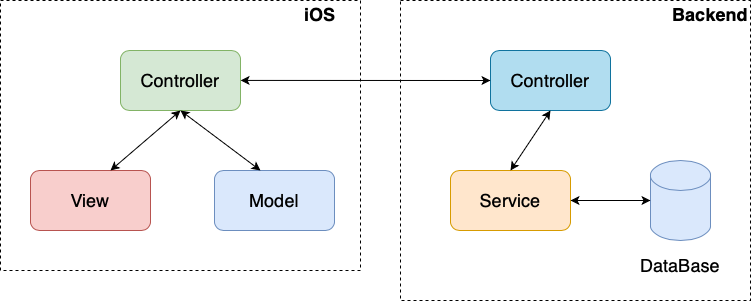
\includegraphics[width=1\linewidth]{Hinhve/Architecture/System_Architecture.png}
    \caption{Kiến trúc tổng quan của hệ thống}
    \label{fig:use_case_tổng_quan}
\end{figure}

Phần BackEnd của hệ thống được xây dựng bằng Vapor-Swift, dựa trên mô hình kiến trúc hướng sự kiện. Phần iOS được xây dựng dựa trên kiến trúc MVC.

Ưu điểm của việc sử dụng kiến trúc hướng sự kiện được sử dụng trong back-end:
\begin{itemize}
    \item Có khả năng chịu tải cao hơn.
    \item Các thành phần trong hệ thống không còn phụ thuộc lẫn nhau.
    \item Khả năng mở rộng tốt.
    \item Phát triển backend nhanh, đơn giản, dễ lập trình, dễ bảo trì.
    \item Dễ dàng kiểm tra: dễ dàng hơn trong việc kiểm tra, rà soát lỗi do các controller được phân tách một cách độc lập.
\end{itemize}
Luồng dữ liệu của mô hình: Người dùng gửi yêu cầu bằng các thao tác trên giao diện, Controller trên iOS client sẽ kiểm tra dữ liệu từ Model và yêu cầu Model đồng bộ dữ liệu với Server, Controller trên Server sẽ nhận được request và giao yêu cầu đến Service tương ứng. Service truy cập vào Database truy vấn và trả về dữ liệu là các Model Object cho Controller. Controller trên server nhận được Model Object sẽ trả về cho Client thông qua lời gọi API. Model trên iOS client Nhận được dữ liệu sẽ gọi hàm CallBack đến Controller trên iOS Client, sau đó Controller cập nhật giao diện.
\newpage

\begin{figure}[H]
    \centering
    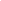
\includegraphics[width=1\linewidth]{Hinhve/Architecture/System_Data_Flow.png}
    \caption{Luồng hoạt động của BackEnd}
    \label{fig:use_case_tổng_quan}
\end{figure}

Mô hình Model-View-Controller (MVC) là một mẫu kiến trúc phân tách một ứng dụng thành ba thành phần logic chính Model, View và Controller. Do đó viết tắt MVC. Mỗi thành phần kiến trúc được xây dựng để xử lý khía cạnh phát triển cụ thể của một ứng dụng. MVC tách lớp logic nghiệp vụ và lớp hiển thị ra riêng biệt. Một số ưu điểm của MCV:
\begin{itemize}
    \item Bảo trì code dễ dàng, dễ dàng mở rộng và phát triển.
    \item Việc phát triển các thành phần khác nhau có thể được thực hiện song song.
    \item Giúp nhà phát triển tránh sự phức tạp bằng cách chia ứng dụng thành ba đơn vị Model, View và Controller.
    \item Cung cấp hỗ trợ tốt nhất cho phát triển theo hướng thử nghiệm.
\end{itemize}
MVC là một mô hình phổ biến và dễ triển khai trong thiết kế xây dựng phần mềm. Ứng dụng được xây dựng dựa trên mô hình MVC được chia làm 3 phần: Model, View, Controller. Mỗi thành phần là độc lập với nhau và có vai trò riêng:
\newline
View:
\begin{itemize}
    \item View là một phần của ứng dụng đại diện cho việc trình bày dữ liệu.
    \item View được tạo bởi các dữ liệu mà chúng ta lấy từ dữ liệu trong model. Một view yêu cầu model cung cấp đầy đủ dữ liệu để nó hiển thị đầu ra cho người dùng.
    \item View chính là nới chứa những giao diện như một nút bấm, vùng nhập dữ liệu từ bàn phím, menu, hình ảnh, nó đảm nhiệm nhiệm vụ hiển thị dữ liệu và giúp người dùng tương tác với hệ thống.
\end{itemize}
Controller:
\begin{itemize}
    \item Controller là một phần của ứng dụng xử lý tương tác của người dùng. Trên iOS, Controller sẽ nhận sự kiện kích hoạt từ View khi người dùng thao tác trên giao diện.
    \item Controller bao gồm những lớp và hàm xử lý nghiệp vụ logic giúp lấy đúng dữ liệu thông tin cần thiết nhờ các nghiệp vụ lớp Model cung cấp và hiển thị dữ liệu đó ra cho người dùng nhờ lớp View.
    \item Controller gửi các lệnh đến model để làm thay đổi trạng thái của nó. Controller cũng gửi các lệnh đến view liên quan của nó để thay đổi cách hiển thị của view.
\end{itemize}
Model:
\begin{itemize}
    \item Thành phần model lưu trữ dữ liệu và logic liên quan của nó. Bao gồm các hàm xử lý các tác vụ như truy vấn, thêm, sửa hoặc xóa dữ liệu. Nó thao tác với dữ liệu trên Server thông qua API hoặc dữ liệu lưu trên thiết bị sau đó sử dụng nó để hiển thị dữ liệu.
\end{itemize}
Sự tương tác giữa các thành phần trong mô hình MVC:
\begin{itemize}
    \item Controller tương tác qua lại với View.
    \item Controller tương tác qua lại với Model.
    \item Model và View không có sự tương tác với nhau trực tiếp mà nó tương tác với nhau thông qua Controller.
\end{itemize}

\begin{figure}[H]
    \centering
    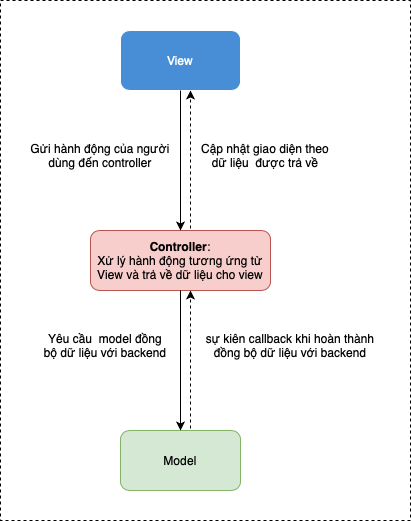
\includegraphics[width=1\linewidth]{Hinhve/Architecture/iOS_Client_Data_Flow.png}
    \caption{Luồng hoạt động của ứng dụng trên iOS theo mô hình MVC}
    \label{fig:use_case_tổng_quan}
\end{figure}



\newpage
\subsection{Thiết kế tổng quan} 
\begin{figure}[H]
    \centering
    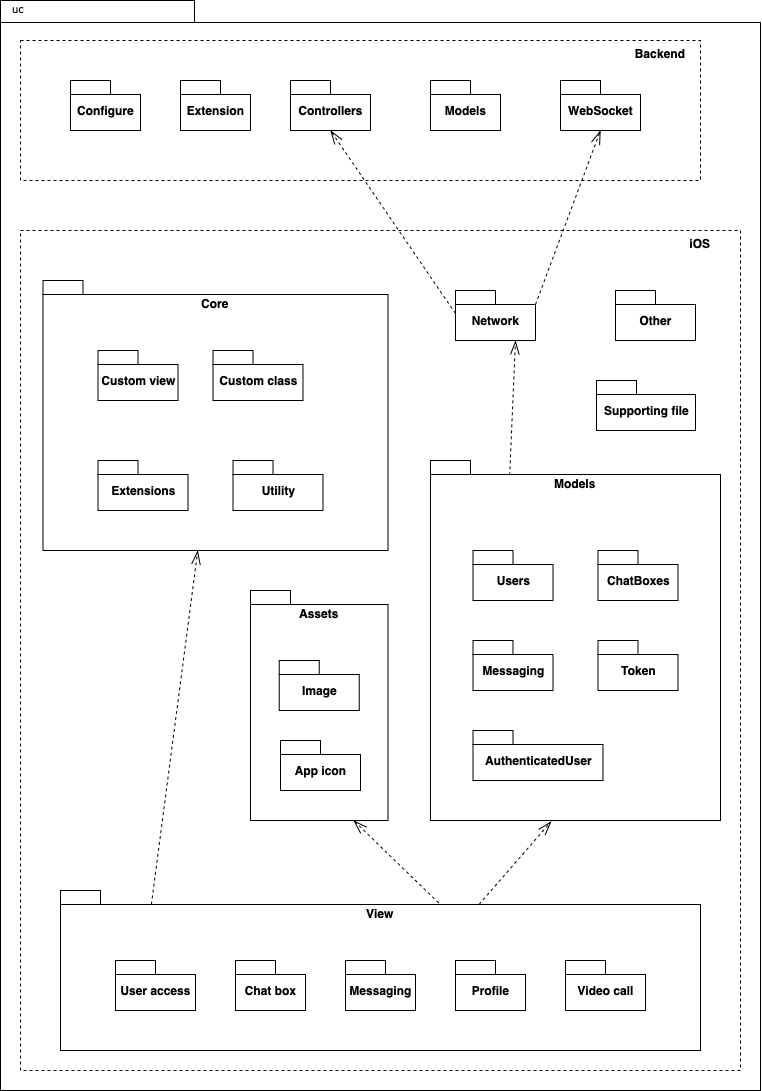
\includegraphics[width=1\linewidth]{Hinhve/Package/Package.png}
    \caption{Thiết kế gói tổng quan}
    \label{fig:use_case_tổng_quan}
\end{figure}
Hệ thống được chia làm 2 thành phần chính: back-end và iOS Client.
Thành phần back-end bao gồm 5 gói chính: (i) Configure, (ii) Extension, (iii) Controllers, (iv) Models, (v) WebSocket: 

\textbf{Gói Configure:} Gói chứa các cấu hình database, cấu hình liên quan đến mạng và cấu hình của server.

\textbf{Gói Extension:} Gói chứa các khai báo mở rộng phương thức cho các class, các kiểu dữ liệu có sẵn.

\textbf{Gói Controllers:} Gói controllers khai báo các class xử lý logic, điều phối lời gọi API.

\textbf{Gói WebSocket:} Gói chứa cái khai báo phục vụ cho việc quản lý Socket cho nhiều người dùng.

Thành phần iOS Client bao gồm 7 gói chính: (i) Core, (ii) Models, (iii) Network, (iv) Assets, (v) View, (vi) Other, (vii) Supporting file: 

\textbf{Gói Core:} Gói chứa các class có thể tái sử dụng trong ứng dụng, như điều khiển phản hồi rung của thiết bị, màn hình loading. Ngoài ra gói chứa các khai bao mở rộng phương thức cho các class, các kiểu dữ liệu có sẵn.

\textbf{Gói Models:} Gói đại diện cho thành phần model trong kiến trúc MVC, cung cấp dữ liệu và khả năng lưu trữ dữ liệu vào bộ nhớ cho ứng dụng.

\textbf{Gói NetWork:} Gói chứa các class có chức năng giao tiếp với server.

\textbf{Gói Assets:} Gói chứa dữ liệu media như ảnh của các button, video, ảnh logo của ứng dụng.

\textbf{Gói View:} Gói đại diện cho thành phần View trong kiến trúc MVC, gói chứa các gói thành phần, mỗi gói thành phần bao gồm View và controller trong nó. Gói có nhiệm vụ hiển thị dữ liệu, tương tác trực tiếp với người dùng cũng như xử lý nghiệp vụ logic.

\textbf{Gói Other:} Chứa các thành phần mà trình biên dịch tự động tạo ra hỗ trợ lập trình viên trong quá trình phát triển phần mềm, như kiểm thử tự động, khai báo quyền truy cập trên thiết bị, vòng đời của phần mềm,..

\textbf{Gói Supporting file:} Chứa các thư viện ngoài, khai báo dữ liệu mẫu,..


\subsection{Thiết kế chi tiết gói Messaging} 
\begin{figure}[H]
    \centering
    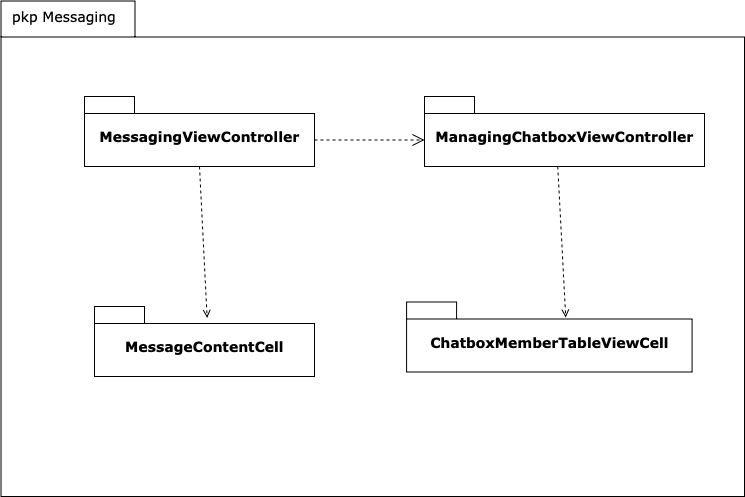
\includegraphics[width=0.9\linewidth]{Hinhve/Package/Messaging_Package_Detail.png}
    \caption{Thiết kế chi tiết gói Messaging}
    \label{fig:use_case_tổng_quan}
\end{figure}
Hình 4.5 mô tả chi tiết gói Messaging. Bao gồm các lớp : (i) MessagingViewController, (ii) ManagingChatboxViewController, (iii) MessageContentCell, (iv) ChatBoxMemberTableViewCell. Trong đó từng lớp có nhiệm vụ sau:
\begin{itemize}
    \item MessagingViewController: Controller xử lý các nghiệp vụ logic gửi tin nhắn và đồng bộ tin nhắn.
    \item ManagingChatboxViewController: Controller xử lý các nghiệp vụ logic thêm thành viên và xoá thành viên khỏi nhóm.
    \item MessageContentCell: View hiển thị tin nhắn văn bản hoặc ảnh.
    \item ChatBoxMemberTableViewCell: View hiển thị người dùng.
\end{itemize} \newpage


\subsection{Thiết kế chi tiết gói User Access} 
\begin{figure}[H]
    \centering
    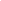
\includegraphics[width=0.9\linewidth]{Hinhve/Package/UserAccess_Package_Detail_iOS_Client.png}
    \caption{Thiết kế chi tiết gói User Access}
    \label{fig:use_case_tổng_quan}
\end{figure}
Hình 4.6 mô tả chi tiết gói User Access. Bao gồm các lớp : (i) SignInViewController, (ii) SignUpViewController, (iii) TextInputCell. Trong đó từng lớp có nhiệm vụ sau:
\begin{itemize}
    \item SignInViewController: Controller xử lý các nghiệp vụ logic màn hình đăng nhập.
    \item SignInViewController.xib: Nơi thiết kế giao diện màn hình đăng nhập.
    \item SignUpViewController: Controller xử lý các nghiệp vụ logic màn hình đăng ký.
    \item SignUpViewController.xib: Nơi thiết kế giao diện màn hình đăng ký.
    \item TextInputCell: Controller xử lý logic hiển thị cho vùng nhập dữ liệu.
    \item TextInputCell.xib: Đối tượng View cho phép nhập dữ liệu từ bàn phím.
\end{itemize} \newpage


\subsection{Thiết kế chi tiết gói Controllers} 
\begin{figure}[H]
    \centering
    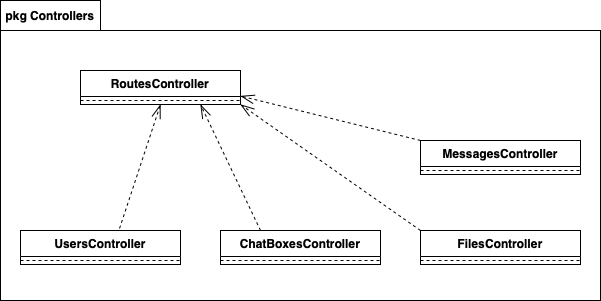
\includegraphics[width=0.9\linewidth]{Hinhve/Package/Controller_Package_Detail_Backend.png}
    \caption{Thiết kế chi tiết gói Controllers}
    \label{fig:use_case_tổng_quan}
\end{figure}
Hình 4.7 mô tả chi tiết gói Controllers. Bao gồm các class: (i) RoutesController, (ii) UsersController, (iii) ChatBoxesController, (iv) MessagesController. Trong đó nhiệm vụ của từng class như sau:
\begin{itemize}
    \item RoutesController: Nơi khai báo class điều phối các Controller. Khi có một yêu cầu từ Client gọi đến, nó sẽ dựa vào đường dẫn và dữ liệu gửi tới để điều phối công việc cho Controller thích hợp.
    \item UsersController: Nơi khai báo class xử lý các nghiệp vụ logic liên quan đến bảng users.
    \item ChatBoxesController: Nơi khai báo class xử lý các nghiệp vụ logic liên quan đến bảng chatBoxes.
    \item MessagesController: Nơi khai báo class xử lý các nghiệp vụ logic liên quan đến bảng messages. 
\end{itemize}\newpage   


\subsection{Thiết kế chi tiết gói Models} 
\begin{figure}[H]
    \centering
    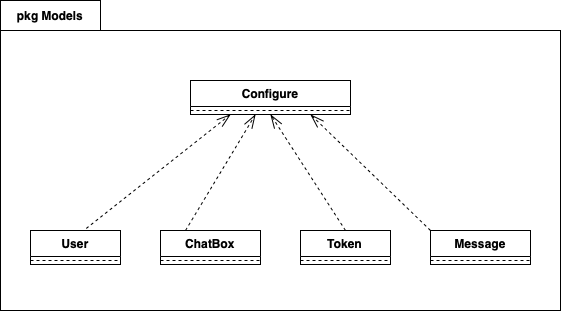
\includegraphics[width=0.9\linewidth]{Hinhve/Package/Models_Package_Detail_Backend.png}
    \caption{Thiết kế chi tiết gói Models}
    \label{fig:use_case_tổng_quan}
\end{figure}
Hình 4.7 mô tả chi tiết gói Models. Bao gồm các struct: (i) User, (ii) ChatBox, (iii) MappingChatBoxPivot, (iv) Message. Trong đó nhiệm vụ của từng class như sau:
\begin{itemize}
    \item User: Nơi khai báo các trường trong bảng users, mỗi đối tượng của struct này thể hiện 1 người dùng.
    \item ChatBox: Nơi khai báo các trường trong bảng chatBoxes, mỗi đối tượng của struct này thể hiện 1 phòng trò chuyện (1 chat box).
    \item MappingChatBoxPivot: Nơi khai báo mối liên hệ giữa 2 bảng users và chatBoxes. Nó thể hiện quan hệ 1 - nhiều giữa bảng users và chatBoxes.
    \item Message: Nơi khai báo các trường trong bảng messages, mỗi đối tượng của struct này thể hiện 1 tin nhắn đã được gửi đi và lưu thành công.
\end{itemize}\newpage



\section{Thiết kế chi tiết}
\subsection{Thiết kế giao diện}
Đối với việc xây dựng, phát triển ứng dụng trên di động, thiết kế giao diện là bước quan trọng. Kết quả của công đoạn thiết kế giao diện quyệt định đến tần suất sử dụng phần mềm, hiệu năng tương tác của người dùng và dựa trên một số yếu tố sau:

Bố cục của ứng dụng: phải được thiết kế phù hợp với nhiều loại màn hình của các phiên bản iPhone. Tỷ lệ, kích thước và vị trí những phần tử hiển thị phải được sắp xếp hợp lý.

Màu sắc: màu sắc giữa các thành phần của ứng dụng phải có sự thống nhất, sử dụng 2 màu chính là trắng và xanh nước biển.

Thiết kế nút bấm: nút bấm sử dụng các icon tượng hình. Các icon được cung cấp bởi Apple. Tất cả các icon đều tuân theo chuẩn Material Design cả về màu sắc lẫn kích thước.

Thứ tự, cấu trúc các màn hình: các màn hình phải được sắp xếp hợp lý, chỉ nên cần tối đa 3 đến 4 chạm (số lần tương tác trên màn hình giao diện) để người dùng thực hiện được mục đích của mình.

Với những màn hình hiển thị dữ liệu từ server trả về, công việc đồng bộ dữ liệu từ server phải được đưa vào luồng phụ, tránh cho giao diện bị giật và không phản hồi lại thao tác người dùng khi sử dụng.



\subsection{Thiết kế lớp}
\subsubsection{Thiết kế chi tiết lớp ChatBoxViewController}
Thiết kế chi tiết lớp ChatBoxViewController được miêu tả như hình vẽ. Lớp ChatBoxViewController phụ thuộc vào 2 lớp là MessagingViewController và ChatBoxModel. ChatBoxViewController hiển thị danh sách các nhóm chat, MessagingViewController hiển thị danh sách các tin nhắn trong 1 nhóm chat cụ thể, ChatBoxModel có nhiệm vụ lấy ra dữ liệu cho ChatBoxViewController hiển thị, sau đó MessagingViewController được ChatBoxViewController gọi đến và lớp MessageModel lấy dữ liệu cho MessagingViewController hiển thị. Lớp MessagingViewController cần tham số đầu vào là chatBoxId để có thể lấy ra những tin nhắn thuộc nhóm chat.
Lớp VideoCallViewController thực hiện nhiệm vụ xử lý logic khi thực hiện gọi video, lớp MessagingViewController gọi đến lớp VideoCallViewController và hiển thị.

\begin{figure}[H]
    \centering
    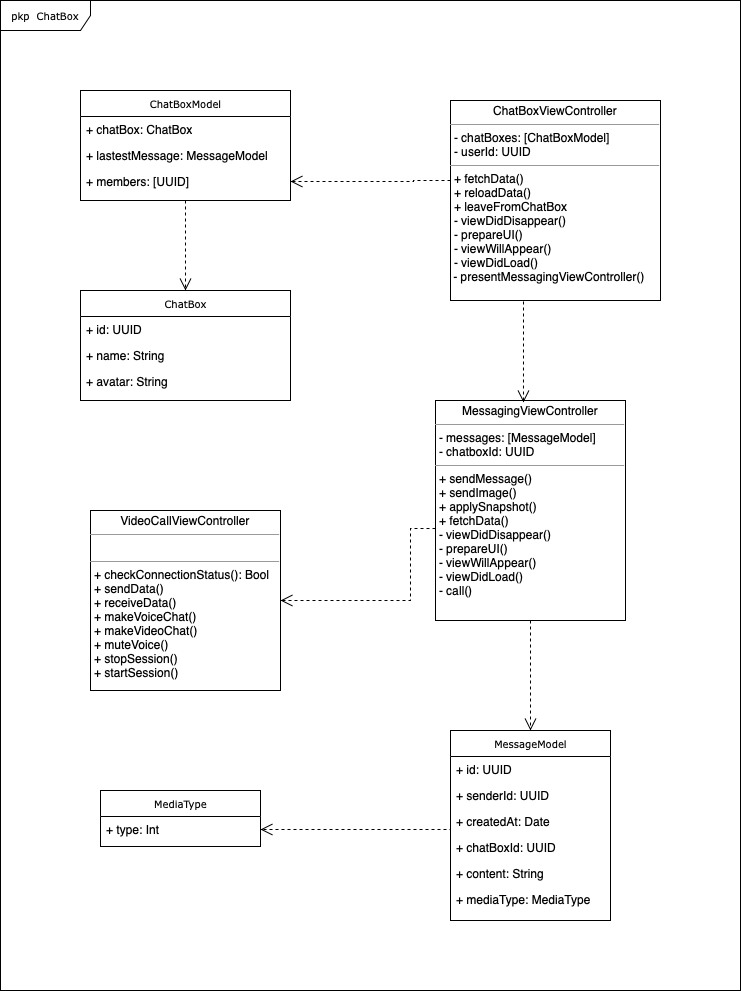
\includegraphics[width=1\linewidth]{Hinhve/Class/Detail_ChatboxViewController_Class_PKP.png}
    \caption{Thiết kế chi tiết lớp ChatBoxViewController}
    \label{fig:use_case_tổng_quan}
\end{figure}

\subsubsection{Thiết kế chi tiết lớp ManagingChatBoxViewController}
Thiết kế chi tiết lớp ManagingChatBoxViewController được miêu tả như hình vẽ. Lớp ManagingChatBoxViewController phụ thuộc vào 2 lớp là MessagingViewController và ChatBoxViewController. ManagingChatBoxViewController có nhiệm vụ hiển thị danh sách thành viên thuộc nhóm và những người dùng không thuộc nhóm, ManagingChatBoxViewController cần tham số đầu vào là danh sách những thành viên thuộc nhóm. Khi sự kiện thêm hoặc xoá người dùng, ManagingChatBoxViewController thông báo đến MessagingViewController và ChatBoxViewController để chúng cập nhật dữ liệu.
\begin{figure}[H]
    \centering
    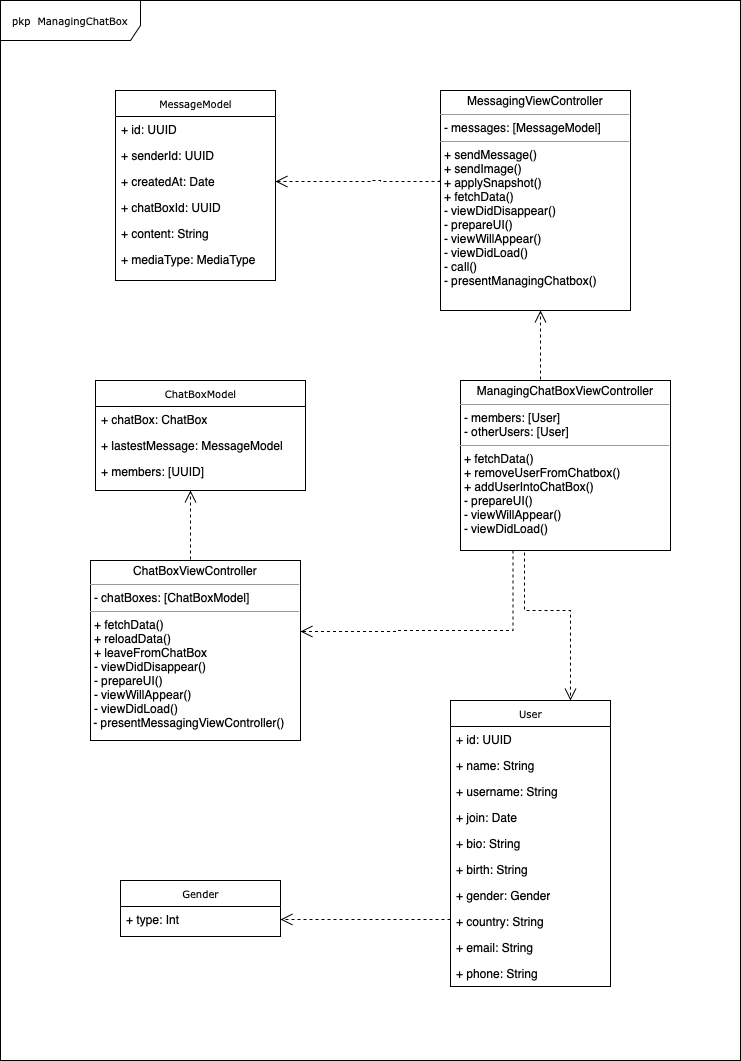
\includegraphics[width=1\linewidth]{Hinhve/Class/Detail_ManagingChatBoxViewController_Class_PKP.png}
    \caption{Thiết kế chi tiết lớp ManagingChatBoxViewController}
    \label{fig:use_case_tổng_quan}
\end{figure}


\subsection{Biểu đồ tuần tự tính năng gọi điện video}
Theo biểu đồ mô tả, khi ứng dụng trên client iOS chạy sẽ tự động gửi ip của mình cho signaling server, nếu 2 client muốn gọi đàm thoại video cho nhau, chúng sẽ gửi yêu cầu lên signaling lên server và lấy về ip của nhau. Khi 2 client có được ip của nhau, kết nối peer–to–peer được tạo ra. Khi đường truyền thiết lập và mở, các luồng media stream được khởi tạo và nhờ đó 2 client iOS gửi dữ liệu media trực tiếp cho nhau.

Media stream là một hình thức stream dữ liệu âm thanh và hình ảnh. Yếu tố này hình thành bằng cách gọi hàm getUserMedia của WebRTC để khởi tạo khi làm việc cục bộ.

Media stream phát huy vai trò cho phép truy cập vào stream của một máy tính. Điều này diễn ra khi một kết nối WebRTC được thiết lập với thiết bị khác.
\begin{figure}[H]
    \centering
    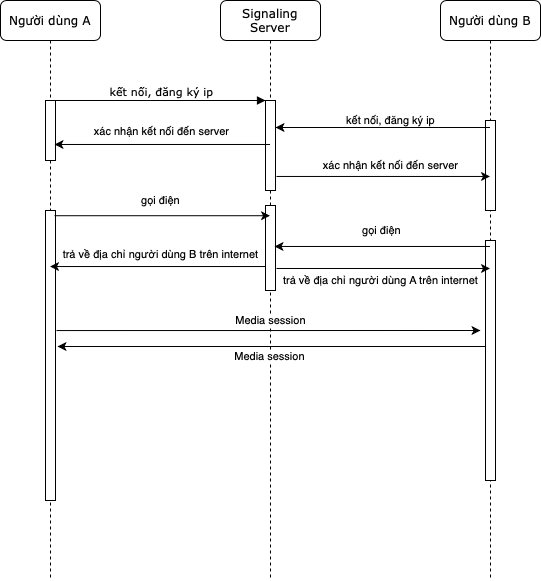
\includegraphics[width=1\linewidth]{Hinhve/Sequence/Sequence_Call_Video.png}
    \caption{Biểu đồ tuần tự tính năng gọi điện video}
    \label{fig:use_case_tổng_quan}
\end{figure}


\subsection{Thiết kế cơ sở dữ liệu}
\begin{figure}[H]
    \centering
    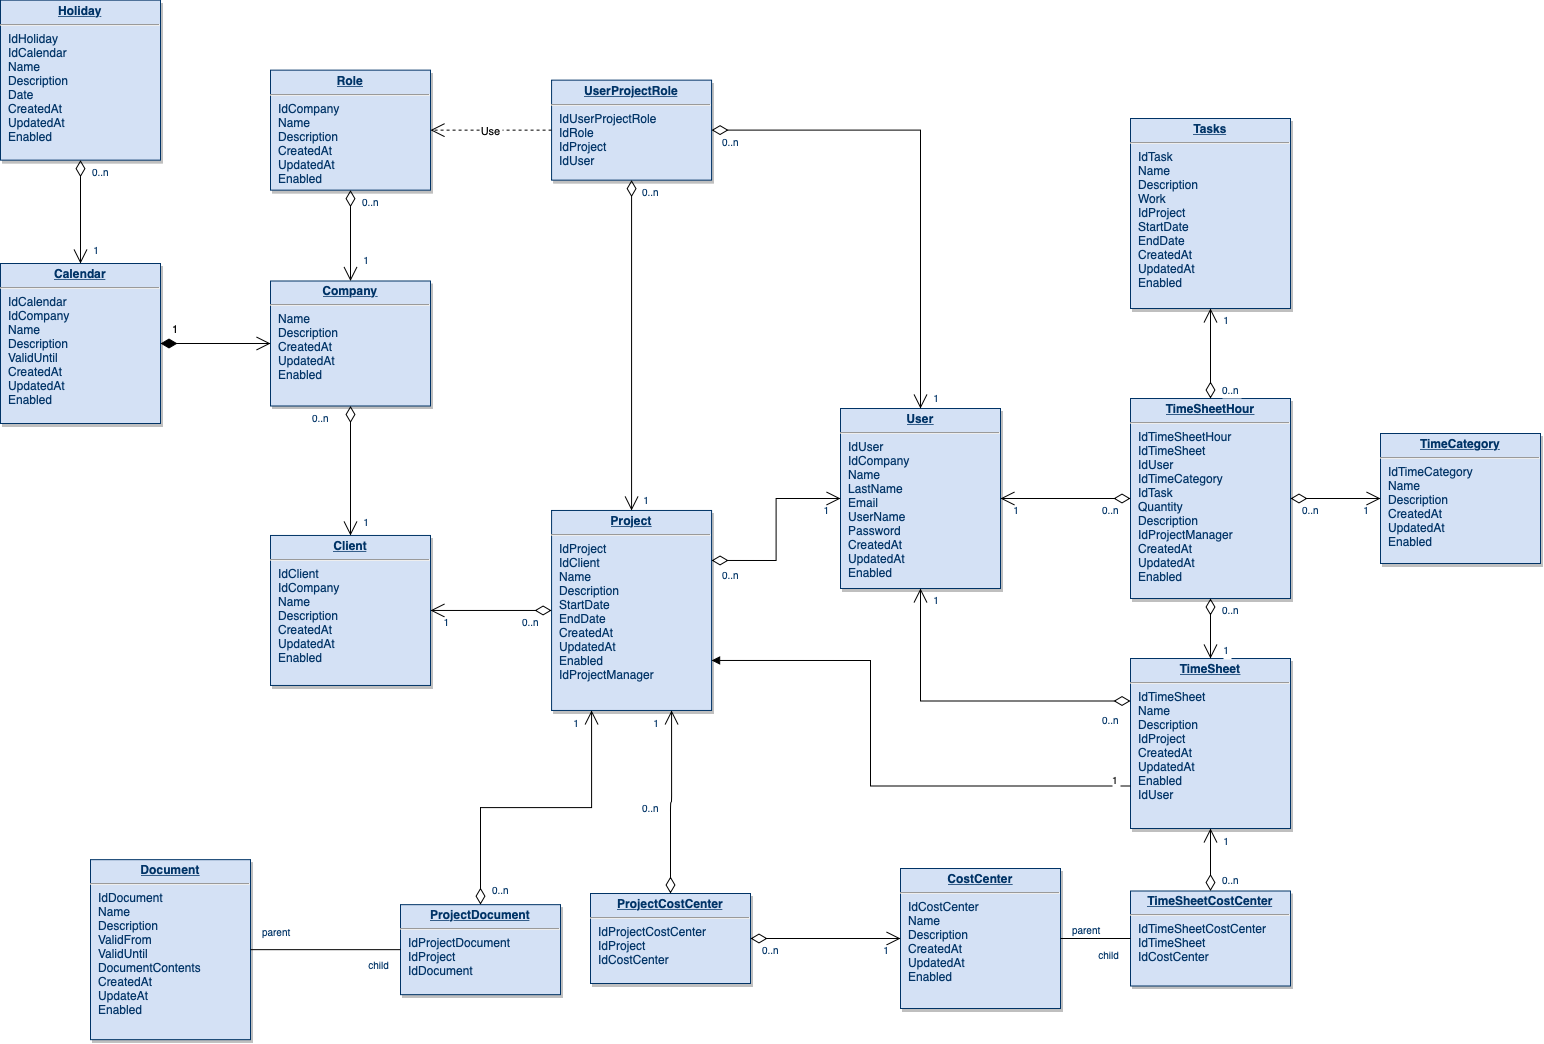
\includegraphics[width=1\linewidth]{Hinhve/Database/Database.png}
    \caption{Sơ đồ thiết kế cơ sở dữ liệu}
    \label{fig:use_case_tổng_quan}
\end{figure}


\newpage
\textbf{Bảng dữ liệu User}

Mục đích: Lưu thông tin của người dùng.

Danh sách thuộc tính:
\begin{longtable}[c]{
|>{\raggedright\arraybackslash}m{0.05\linewidth}
|>{\raggedright\arraybackslash}m{0.15\linewidth}
|>{\raggedright\arraybackslash}m{0.20\linewidth}
|>{\raggedright\arraybackslash}m{0.25\linewidth}
|>{\raggedright\arraybackslash}m{0.1\linewidth}
|>{\raggedright\arraybackslash}m{0.15\linewidth}|}
\hline
\textbf{Thứ tự} & \textbf{Tên} & \textbf{Kiểu dữ liệu} & \textbf{Mô tả} & \textbf{Có bắt buộc} & \textbf{Có ràng buộc} \hline
\endfirsthead
1 & id & UUID & Id của người dùng & Có & Khoá chính \\ \hline
2 & name & Varchar(255) & Tên của người dùng & Có & \\ \hline
3 & username & Varchar(255) & Tên năng nhập của người dùng & Có & Duy nhất \\ \hline
4 & password & Varchar(255) & Mật khẩu & Có & \\ \hline
5 & gender & Varchar(255) & giới tính của người dùng & Không & \\ \hline
6 & bio & Varchar(255) & Thông tin giới thiệu bản thân của người dùng & Không & \\ \hline
7 & birth & Varchar(255) & Ngày tháng năm sinh của người dùng & Không & \\ \hline
8 & phone & Varchar(255) & Số điện thoại của người dùng & Không & \\ \hline
9 & email & Varchar(255) & Email của người dùng & Không & \\ \hline
10 & country & Varchar(255) & Quốc gia của người dùng & Không &  \\ \hline
11 & join & Date & Quốc gia của người dùng & Không & \\ \hline
12 & avatar & Varchar(255) & Quốc gia của người dùng & Không & \\ \hline
\caption{Bảng dữ liệu User}
\label{tab:use_case_tổng_quan}
\end{longtable}
% \begin{figure}[H]
%     \centering
%     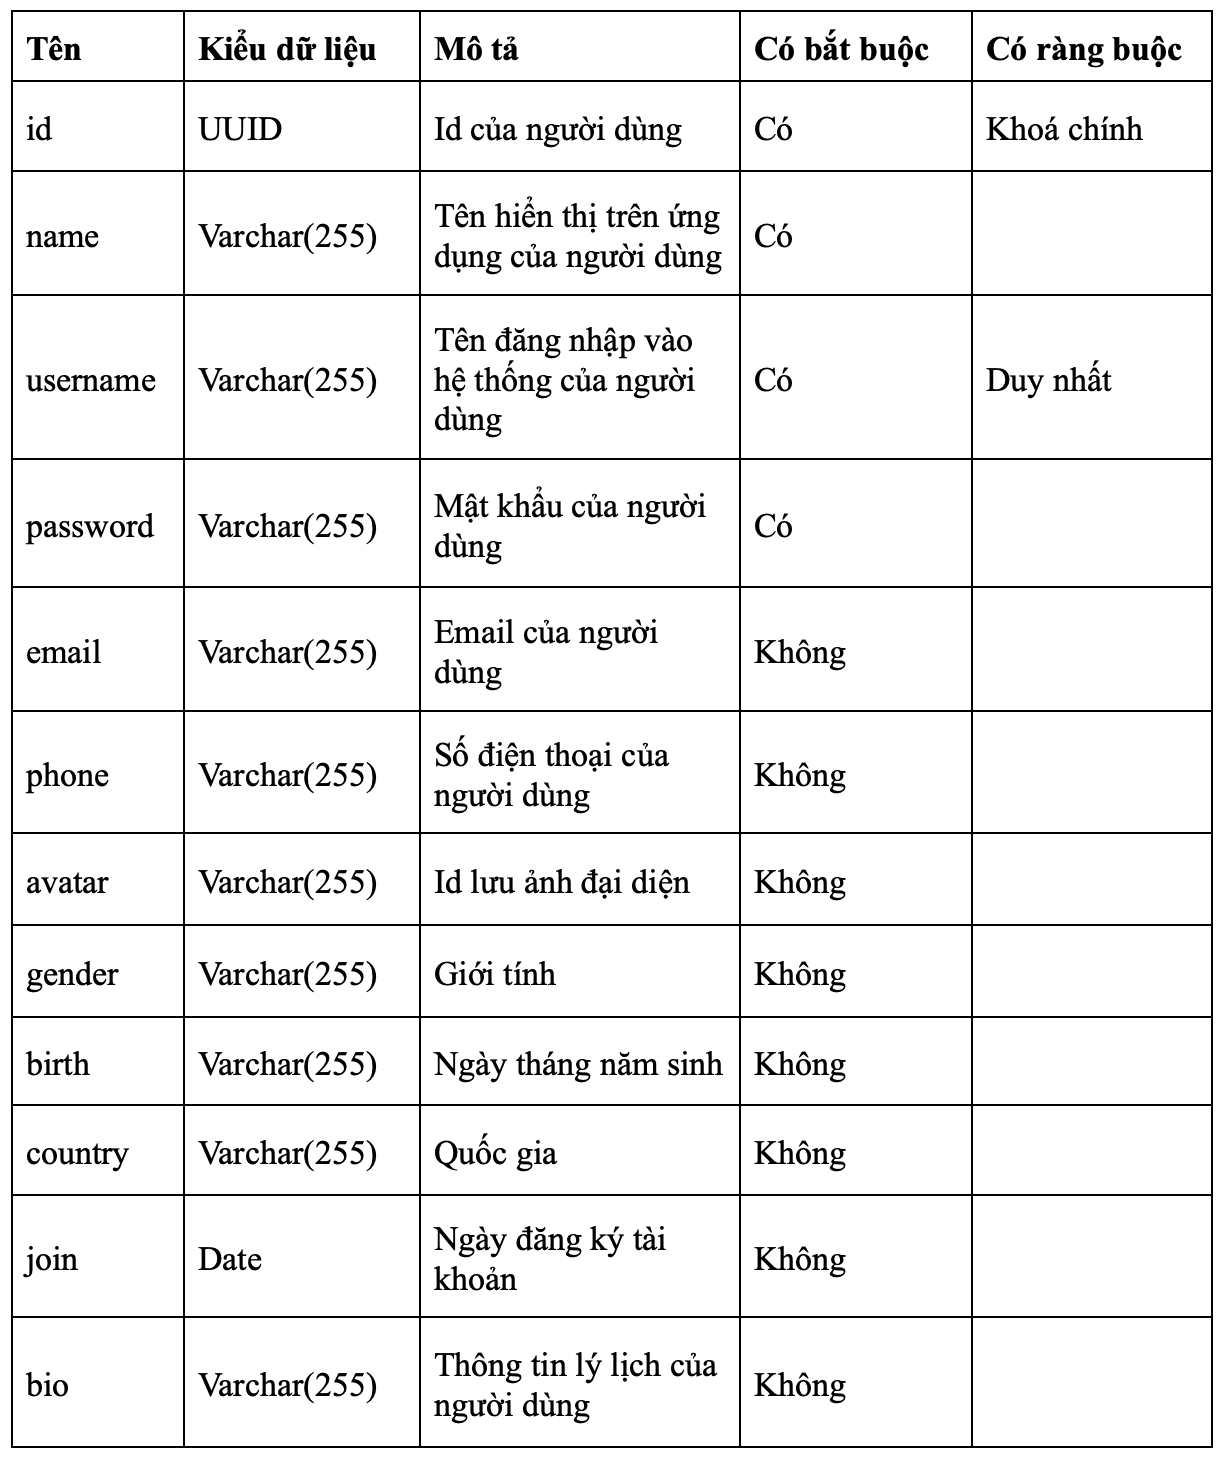
\includegraphics[width=1\linewidth]{Hinhve/Database/Users_Table.png}
%     \caption{Bảng dữ liệu User}
%     \label{fig:use_case_tổng_quan}
% \end{figure}


\newpage
\textbf{Bảng dữ liệu Chatbox}

Mục đích: Lưu thông tin phòng chat.

Danh sách thuộc tính:
\begin{longtable}[c]{
|>{\raggedright\arraybackslash}m{0.05\linewidth}
|>{\raggedright\arraybackslash}m{0.15\linewidth}
|>{\raggedright\arraybackslash}m{0.20\linewidth}
|>{\raggedright\arraybackslash}m{0.25\linewidth}
|>{\raggedright\arraybackslash}m{0.1\linewidth}
|>{\raggedright\arraybackslash}m{0.15\linewidth}|}
\hline
\textbf{Thứ tự} & \textbf{Tên} & \textbf{Kiểu dữ liệu} & \textbf{Mô tả} & \textbf{Có bắt buộc} & \textbf{Có ràng buộc} \hline
\endfirsthead
1 & id & UUID & Id chatbox (id của phòng chat) & Có & Khoá chính \\ \hline
2 & name & Varchar(255) & Tên chatbox (tên của phòng chat) & Không & \\ \hline
3 & avartar & Varchar(255) & Id lưu ảnh đại diện chatbox & Không & \\ \hline
\caption{Bảng dữ liệu Chatbox}
\label{tab:use_case_tổng_quan}
\end{longtable}
% \begin{figure}[H]
%     \centering
%     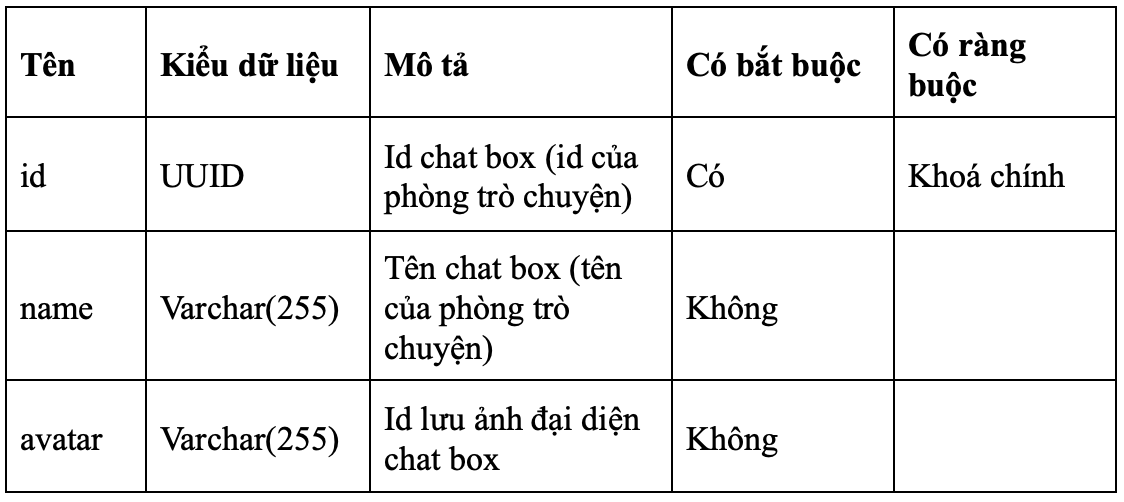
\includegraphics[width=1\linewidth]{Hinhve/Database/Chatboxes_Table.png}
%     \caption{Bảng dữ liệu Chatbox}
%     \label{fig:use_case_tổng_quan}
% \end{figure}


\textbf{Bảng dữ liệu Message}

Mục đích: Lưu tin nhắn của các phòng chat.

Danh sách thuộc tính:
\begin{longtable}[c]{
|>{\raggedright\arraybackslash}m{0.05\linewidth}
|>{\raggedright\arraybackslash}m{0.15\linewidth}
|>{\raggedright\arraybackslash}m{0.20\linewidth}
|>{\raggedright\arraybackslash}m{0.25\linewidth}
|>{\raggedright\arraybackslash}m{0.1\linewidth}
|>{\raggedright\arraybackslash}m{0.15\linewidth}|}
\hline
\textbf{Thứ tự} & \textbf{Tên} & \textbf{Kiểu dữ liệu} & \textbf{Mô tả} & \textbf{Có bắt buộc} & \textbf{Có ràng buộc} \hline
\endfirsthead
1 & id & UUID & Id của tin nhắn & Có & Khoá chính \\ \hline
2 & created\_at & Date & Ngày tin nhắn được gửi & Có & \\ \hline
3 & sender & UUID & Id người gửi tin nhắn & Có & \\ \hline
4 & media\_type & Varchar(255) & Kiểu dữ liệu của tin nhắn & Có & \\ \hline
5 & content & Varchar(255) & Nội dung tin nhắn & Có & \\ \hline
6 & chatbox\_id & Varchar(255) & Id chatbox (id của phòng chat) & Có & \\ \hline
\caption{Bảng dữ liệu User}
\label{tab:use_case_tổng_quan}
\end{longtable}
% \begin{figure}[H]
%     \centering
%     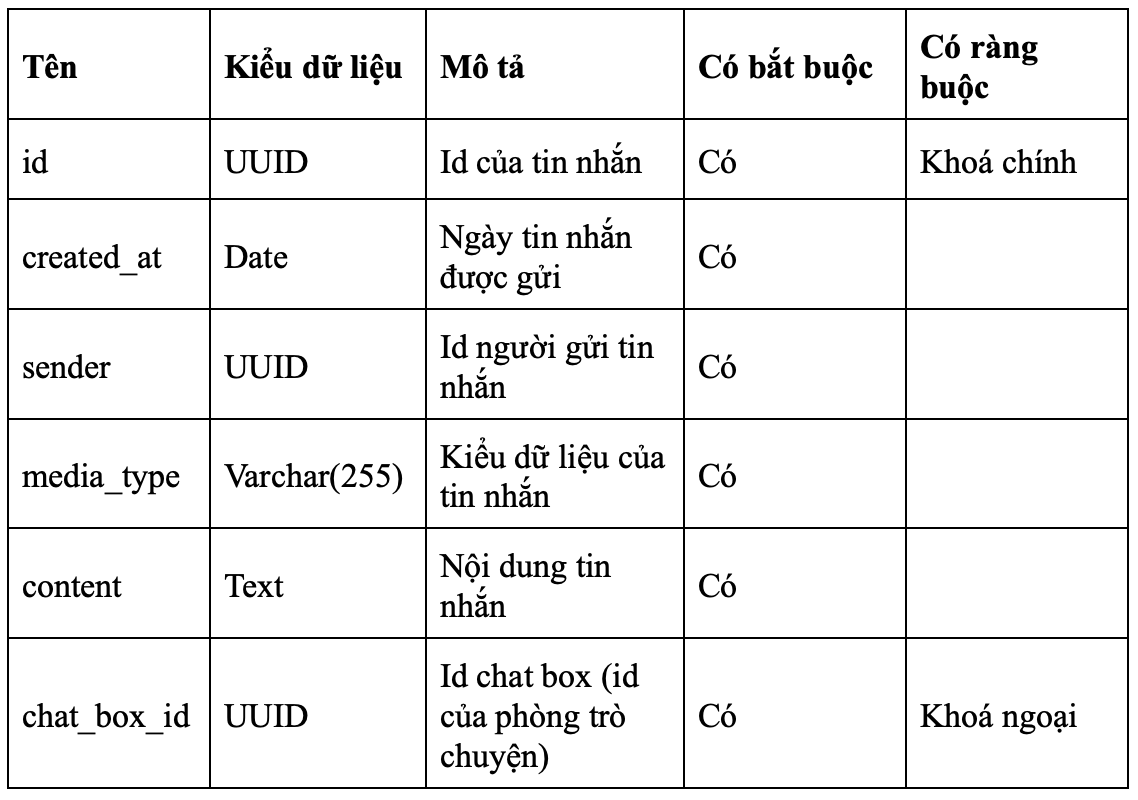
\includegraphics[width=1\linewidth]{Hinhve/Database/Messages_Table.png}
%     \caption{Bảng dữ liệu Message}
%     \label{fig:use_case_tổng_quan}
% \end{figure}


\newpage
\textbf{Bảng dữ liệu Member Of Chatbox}

Mục đích: Lưu id thành viên trong phòng chat.

Danh sách thuộc tính:
\begin{longtable}[c]{
|>{\raggedright\arraybackslash}m{0.05\linewidth}
|>{\raggedright\arraybackslash}m{0.15\linewidth}
|>{\raggedright\arraybackslash}m{0.20\linewidth}
|>{\raggedright\arraybackslash}m{0.25\linewidth}
|>{\raggedright\arraybackslash}m{0.1\linewidth}
|>{\raggedright\arraybackslash}m{0.15\linewidth}|}
\hline
\textbf{Thứ tự} & \textbf{Tên} & \textbf{Kiểu dữ liệu} & \textbf{Mô tả} & \textbf{Có bắt buộc} & \textbf{Có ràng buộc} \hline
\endfirsthead
1 & id & UUID & Id trường dữ liệu & Có & Khoá chính \\ \hline
2 & user\_id & UUID & Id của người dùng & Có & \\ \hline
3 & chatbox\_id & UUID & Id chatbox (id của phòng chat) & Có & \\ \hline
\caption{Bảng dữ liệu members\_of\_chatbox}
\label{tab:use_case_tổng_quan}
\end{longtable}
% \begin{figure}[H]
%     \centering
%     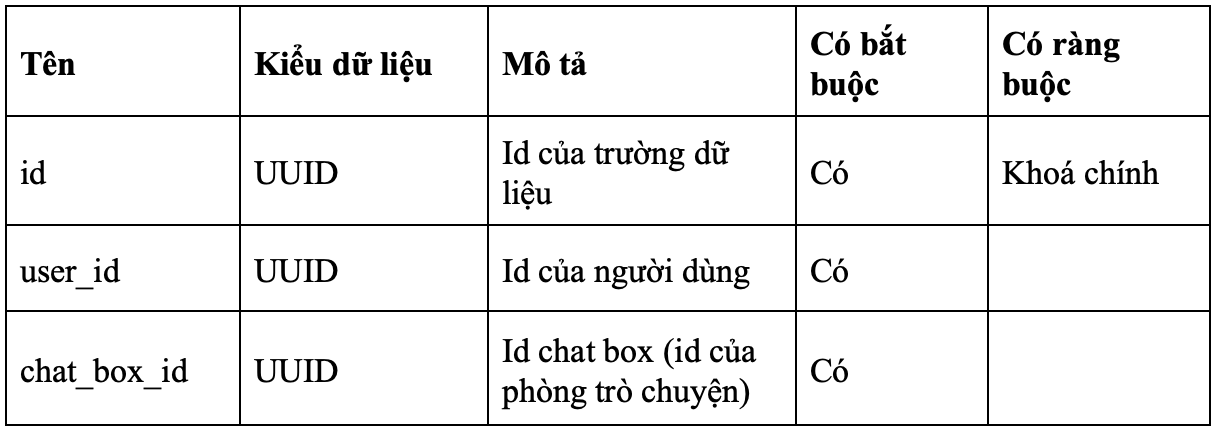
\includegraphics[width=1\linewidth]{Hinhve/Database/Members_Of_Chatbox_Table.png}
%     \caption{Bảng dữ liệu Pivot}
%     \label{fig:use_case_tổng_quan}
% \end{figure}

\section{Xây dựng ứng dụng}
\subsection{Thư viện và công cụ sử dụng}
Các thư viện và công cụ sử dụng để xây dựng đề tài "Phần mềm nhắn tin, gọi điện video trực tuyến":
\begin{longtable}[c]{
|>{\raggedright\arraybackslash}m{0.2\linewidth}
|>{\raggedright\arraybackslash}m{0.3\linewidth}
|>{\raggedright\arraybackslash}m{0.3\linewidth}|}
\hline
\textbf{Công cụ} & \textbf{Mục đích} & \textbf{Địa chỉ URL} \hline
\endfirsthead
Swift & Ngôn ngữ lập trình back-end và iOS & https://developer.apple.c om/swift/ \\ \hline
Visual Code & IDE lập trình & https://code.visualstudi o.com \\ \hline
Xcode & IDE lập trình & https://developer.apple.c om/xcode/ \\ \hline
PostgreSQL & Hệ quản trị cơ sở dữ liệu quan hệ & https://www.postgresql .org \\ \hline
MongoDB & Hệ quản trị cơ sở dữ liệu phi cấu trúc & https://www.mongodb.c om \\ \hline
Vapor & Framework lập trình back-end & https://vapor.codes \\ \hline
UIKit & Framework xây dựng giao diện & https://developer.apple.c om/documentation/uikit \\ \hline
Alamofire & Framework hỗ trợ request API & https://github.com/Alam ofire/Alamofire \\ \hline
Nuke & Framework hỗ trợ xử lý ảnh bất đồng bộ, cache ảnh vào bộ nhớ trên thiết bị,.. & https://github.com/kean /Nuke \\ \hline
Combine & Framework của Apple hỗ trợ xử lý bất đồng bộ, đa luồng,.. & https://developer.apple.c om/documentation/combine \\ \hline
StarScream & Framework hỗ trợ WebSocket & https://github.com/dalto niam/Starscream \\ \hline
WebRTC & Framework hỗ trợ xây dựng tính năng gọi điện video trực tuyến & https://webrtc.org \\ \hline
Docker & Tạo môi trường để chạy Vapor, PostgreSQL, MongoDB & https://www.docker.com \\ \hline
\caption{Bảng danh sách thư viện và công cụ sử dụng}
\label{tab:use_case_tổng_quan}
\end{longtable}

% \begin{figure}[H]
%     \centering
%     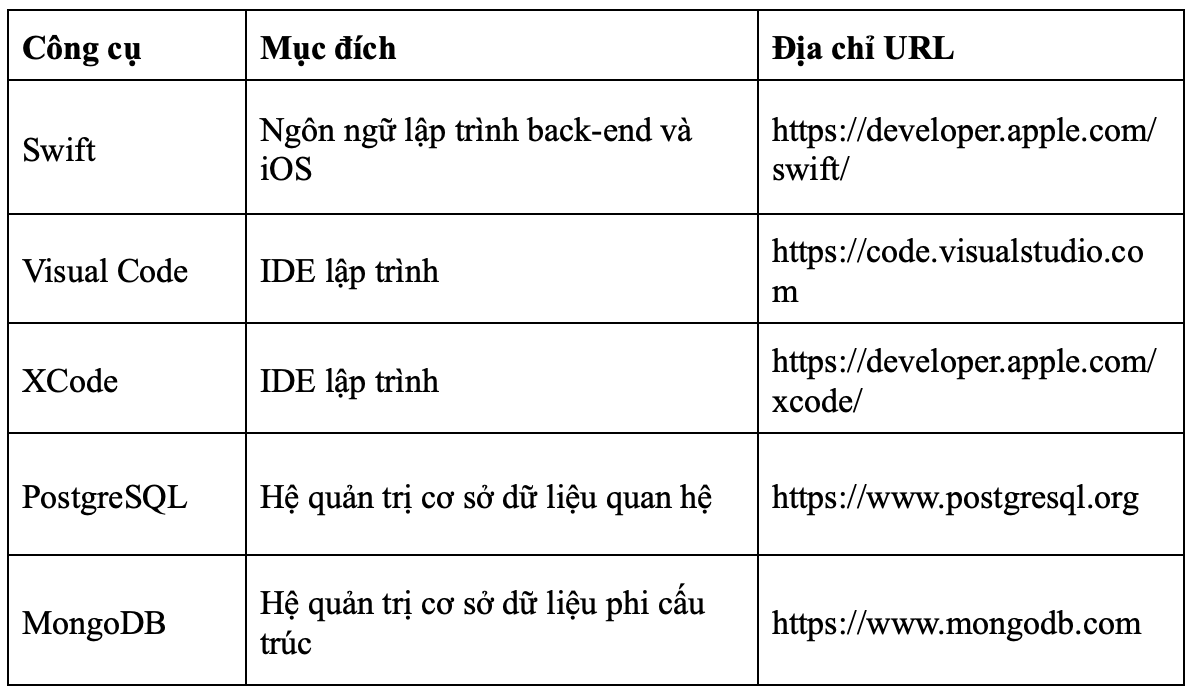
\includegraphics[width=1\linewidth]{Hinhve/Technical_Stack/Technical_Stack_1.png}
% \end{figure}

% \newpage
% \begin{figure}[H]
%     \centering
%     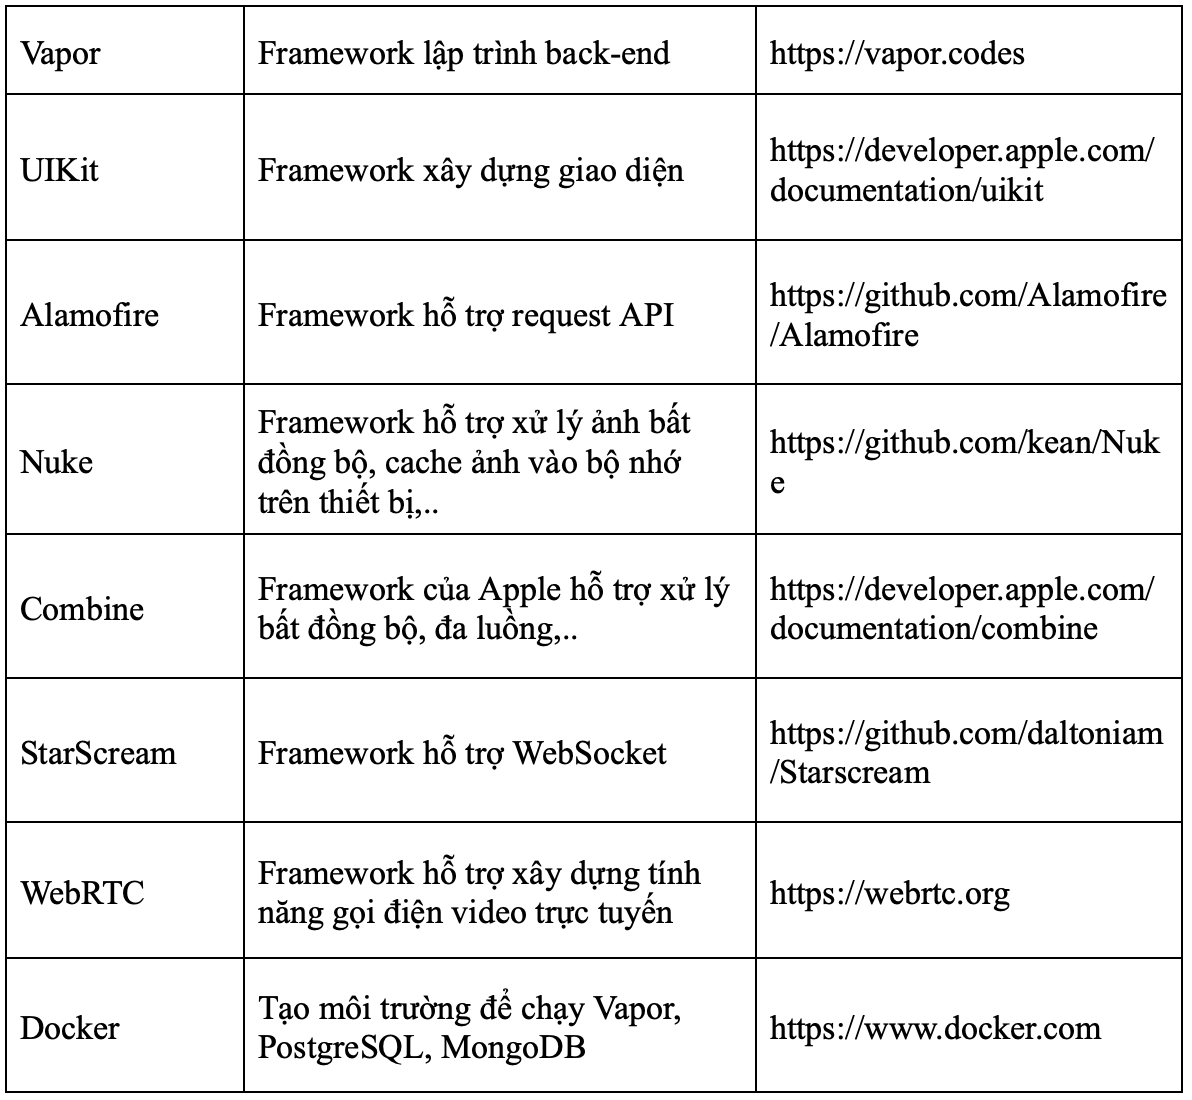
\includegraphics[width=1\linewidth]{Hinhve/Technical_Stack/Technical_Stack_2.png}
%     \caption{Danh sách thư viện và công cụ sử dụng}
%     \label{fig:use_case_tổng_quan}
% \end{figure}


\subsection{Kết quả đạt được}
\begin{longtable}[c]{
|>{\raggedright\arraybackslash}m{0.25\linewidth}
|>{\raggedright\arraybackslash}m{0.25\linewidth}
|>{\raggedright\arraybackslash}m{0.25\linewidth}
|>{\raggedright\arraybackslash}m{0.25\linewidth}|}
\hline
\textbf{Mô tả} & \textbf{Thông tin} \hline
\endfirsthead
Số dòng code & 13950 \\ \hline
Số lượng lớp & 116 \\ \hline
Số giao diện & 12 \\ \hline
Dụng lượng mã nguồn và tài nguyên & 13.8MB \\ \hline
Môi trường lập trình & MacOS \\ \hline
\caption{Thông tin kết quả đạt được}
\label{tab:use_case_tổng_quan}
\end{longtable}

\subsection{Minh hoạ các chức năng chính}
Kết quả đạt được là xây dựng thành công một ứng dụng nhắn tin và gọi diện video trực truyến trên nền tảng iOS và http server trên nền tảng MacOS với các chức năng cơ bản:

Người dùng có thể thể tạo tài khoản và đăng nhập vào hệ thống.

Người dùng đã đăng nhập có thể xem được thông tin công khai của những người dùng khác, chỉnh sửa thông tin cá nhân của bản thân, tạo phòng chat và nhắn tin hoặc gọi điện video với người dùng khác. Ngoài ra người dùng đã đăng nhập có thể tạo nhóm chat và có thể quản lý thành viên trong nhóm.

Người dùng có thể gửi đi tin nhắn là văn bản hoặc ảnh.

Hình ảnh minh hoạ sử dụng ứng dụng:

\begin{figure}[H]
\begin{minipage}{0.5\textwidth}
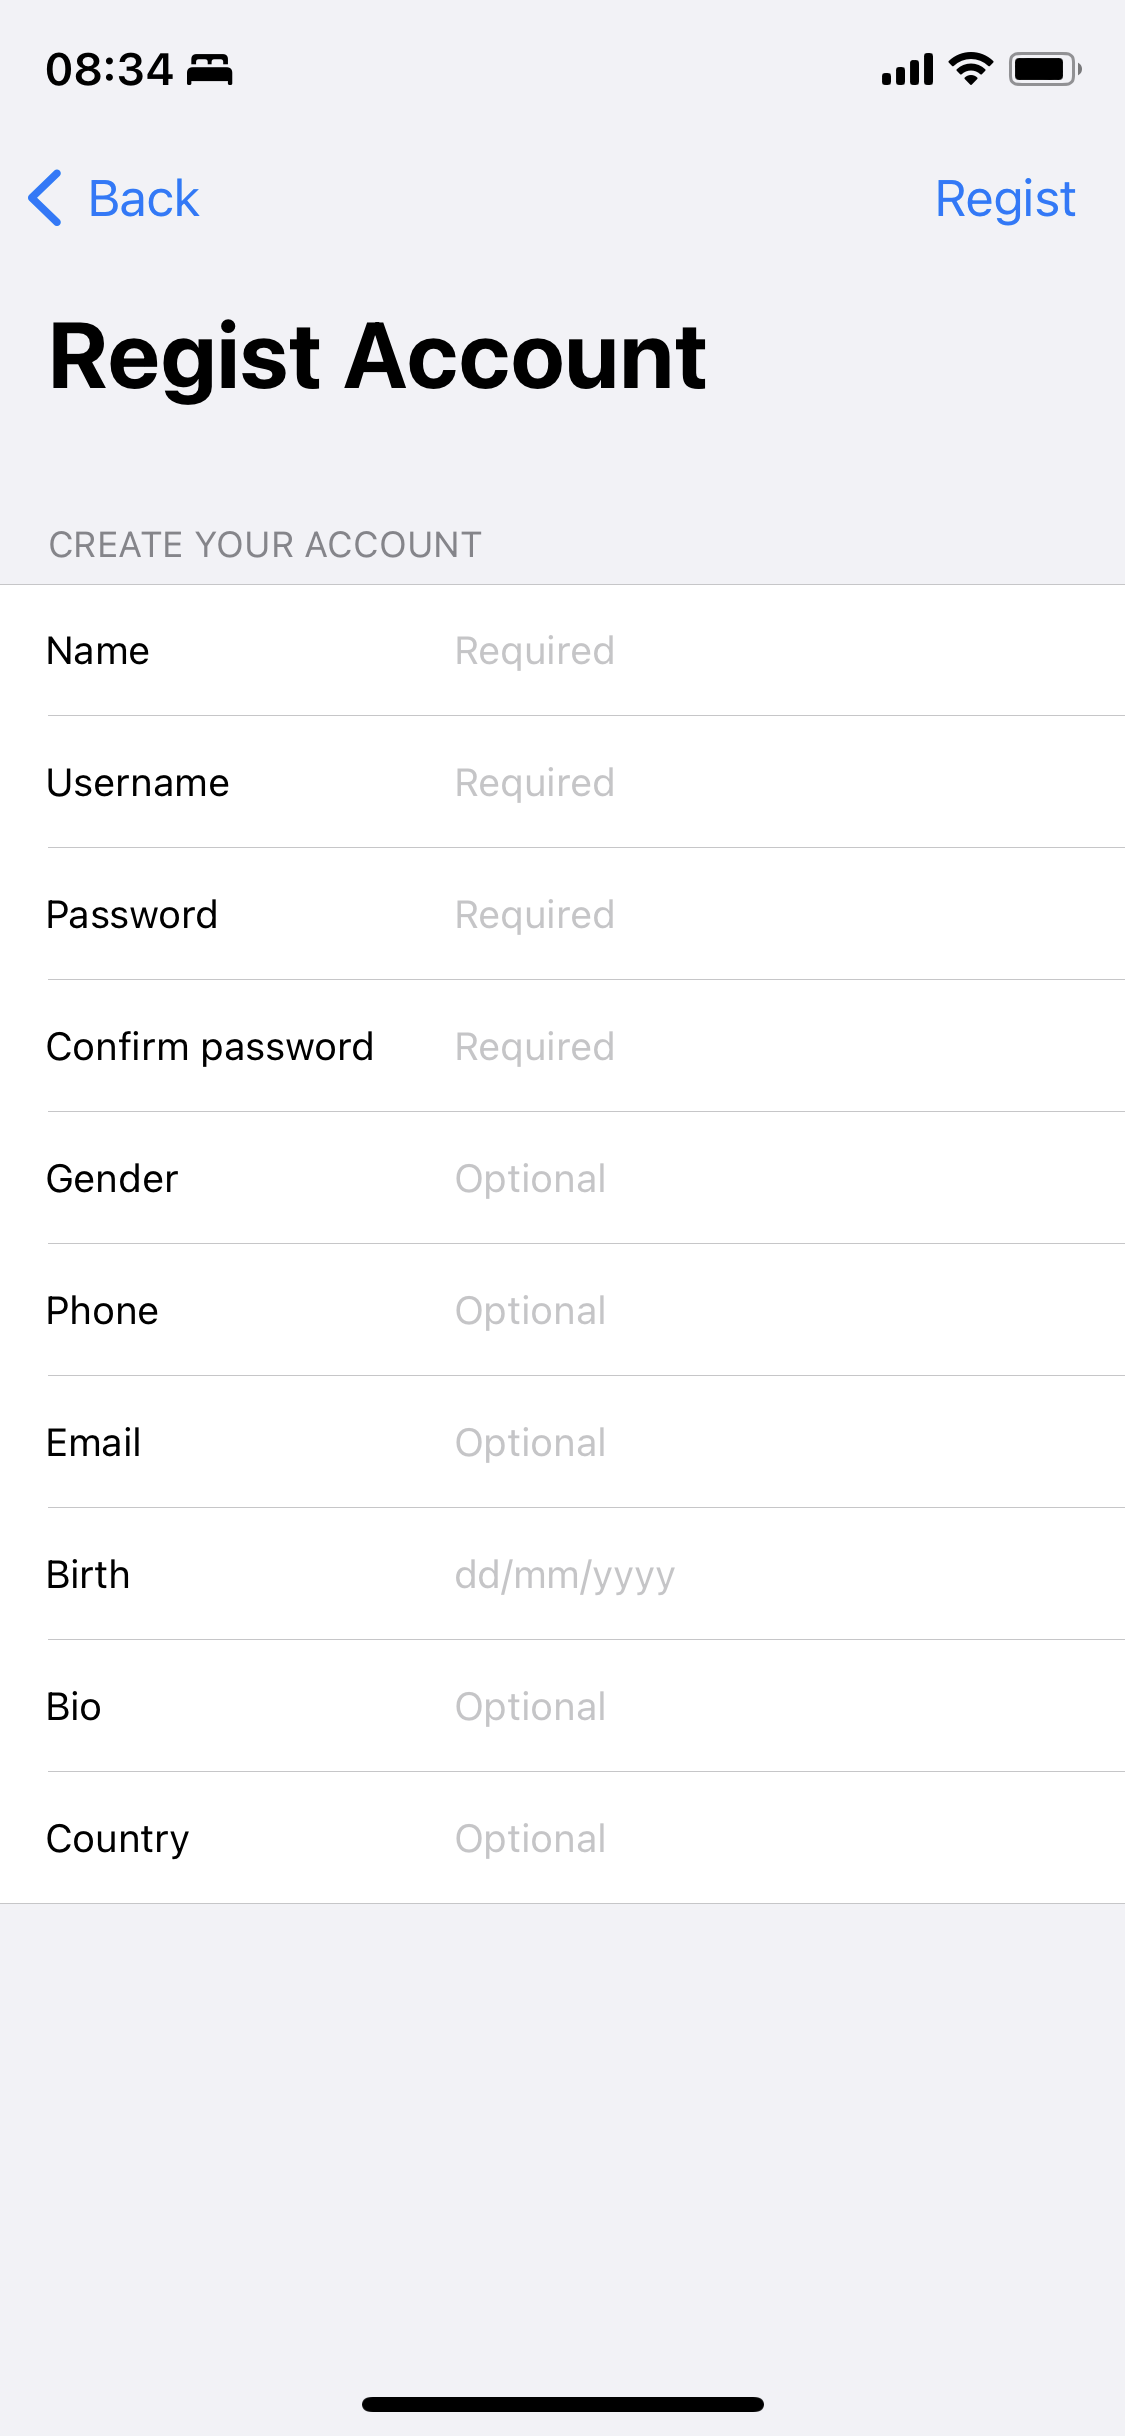
\includegraphics[width=0.95\linewidth]{Hinhve/Application/SignUp.png}
\caption{Màn hình đăng ký} \label{fig:screen_login}
\end{minipage}
\hspace{\fill}
\begin{minipage}{0.5\textwidth}
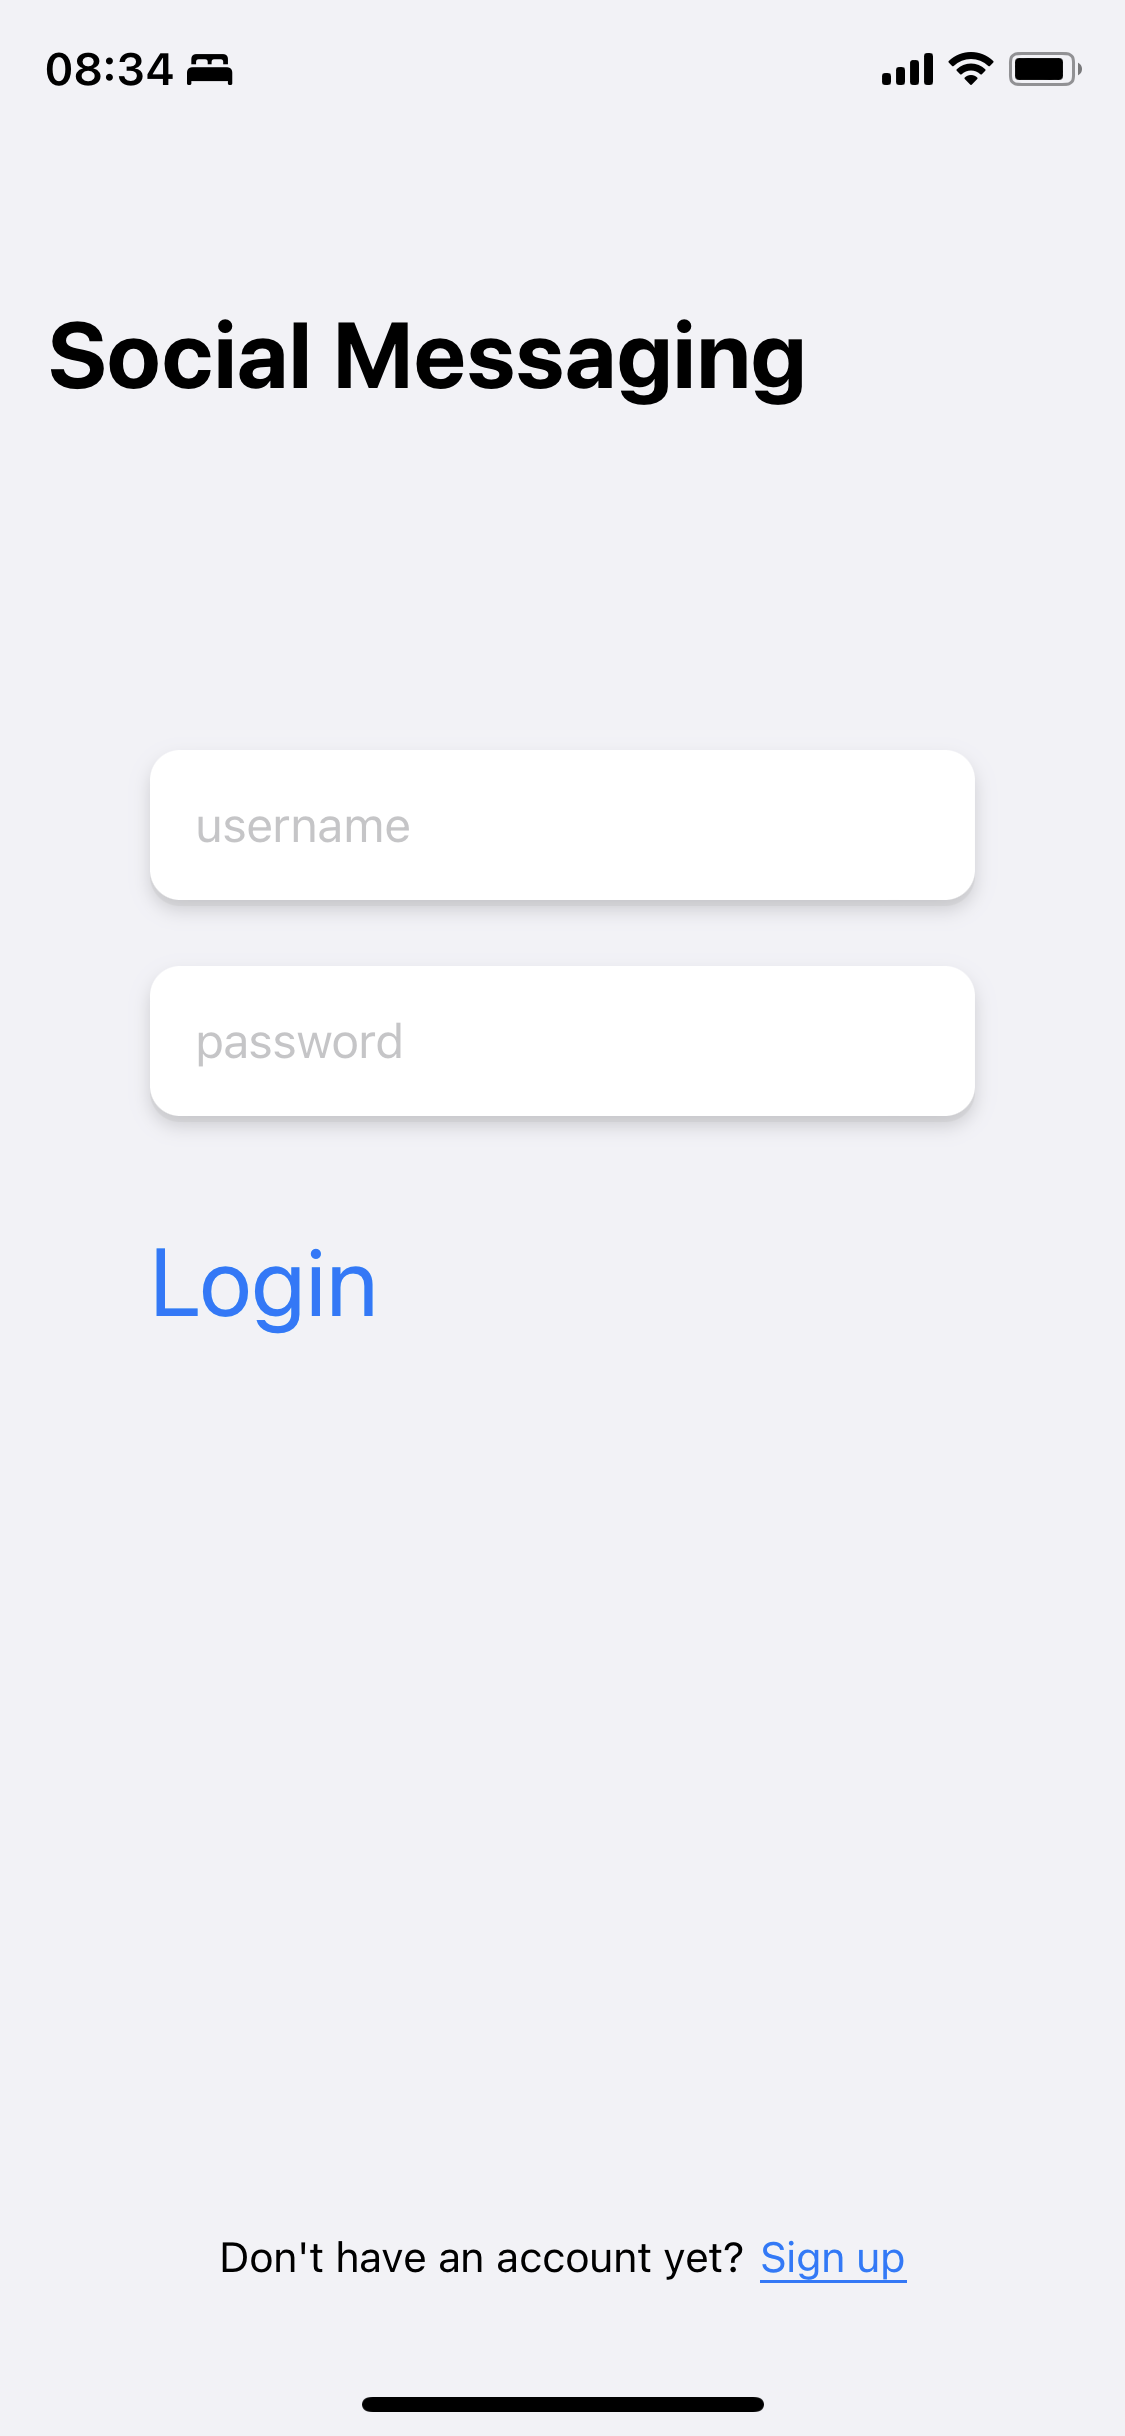
\includegraphics[width=0.95\linewidth]{Hinhve/Application/SignIn.png}
\caption{Màn hình đăng nhập} \label{fig:list_task}
\end{minipage}
\end{figure}
\hfill

\begin{figure}[H]
\begin{minipage}{0.5\textwidth}
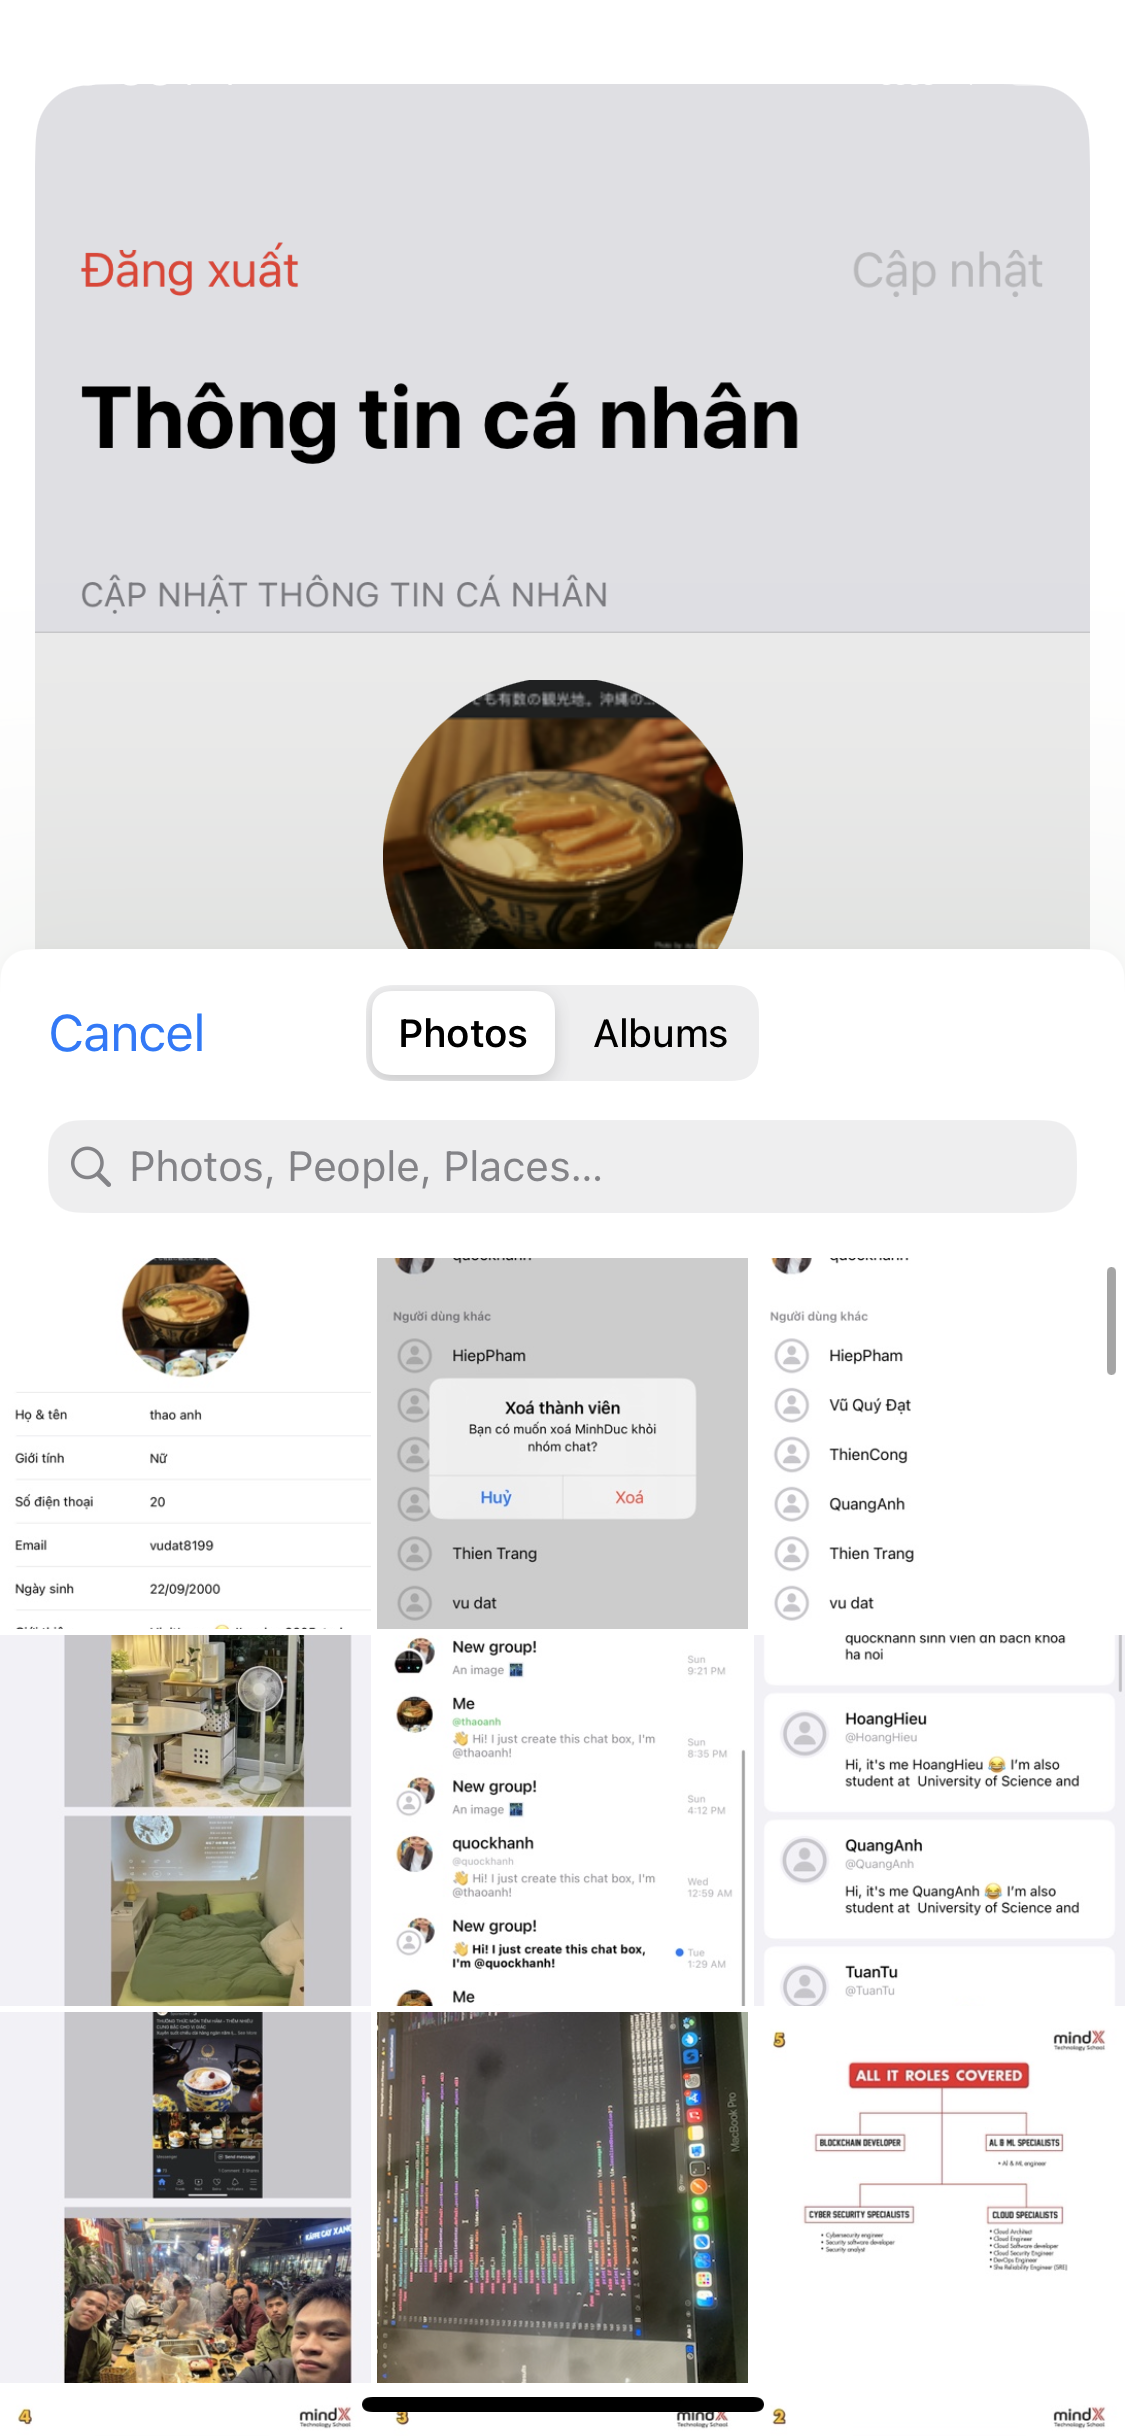
\includegraphics[width=0.95\linewidth]{Hinhve/Application/Change_Avatar.png}
\caption{Màn hình thay đổi avatar} \label{fig:screen_login}
\end{minipage}
\hspace{\fill}
\begin{minipage}{0.5\textwidth}
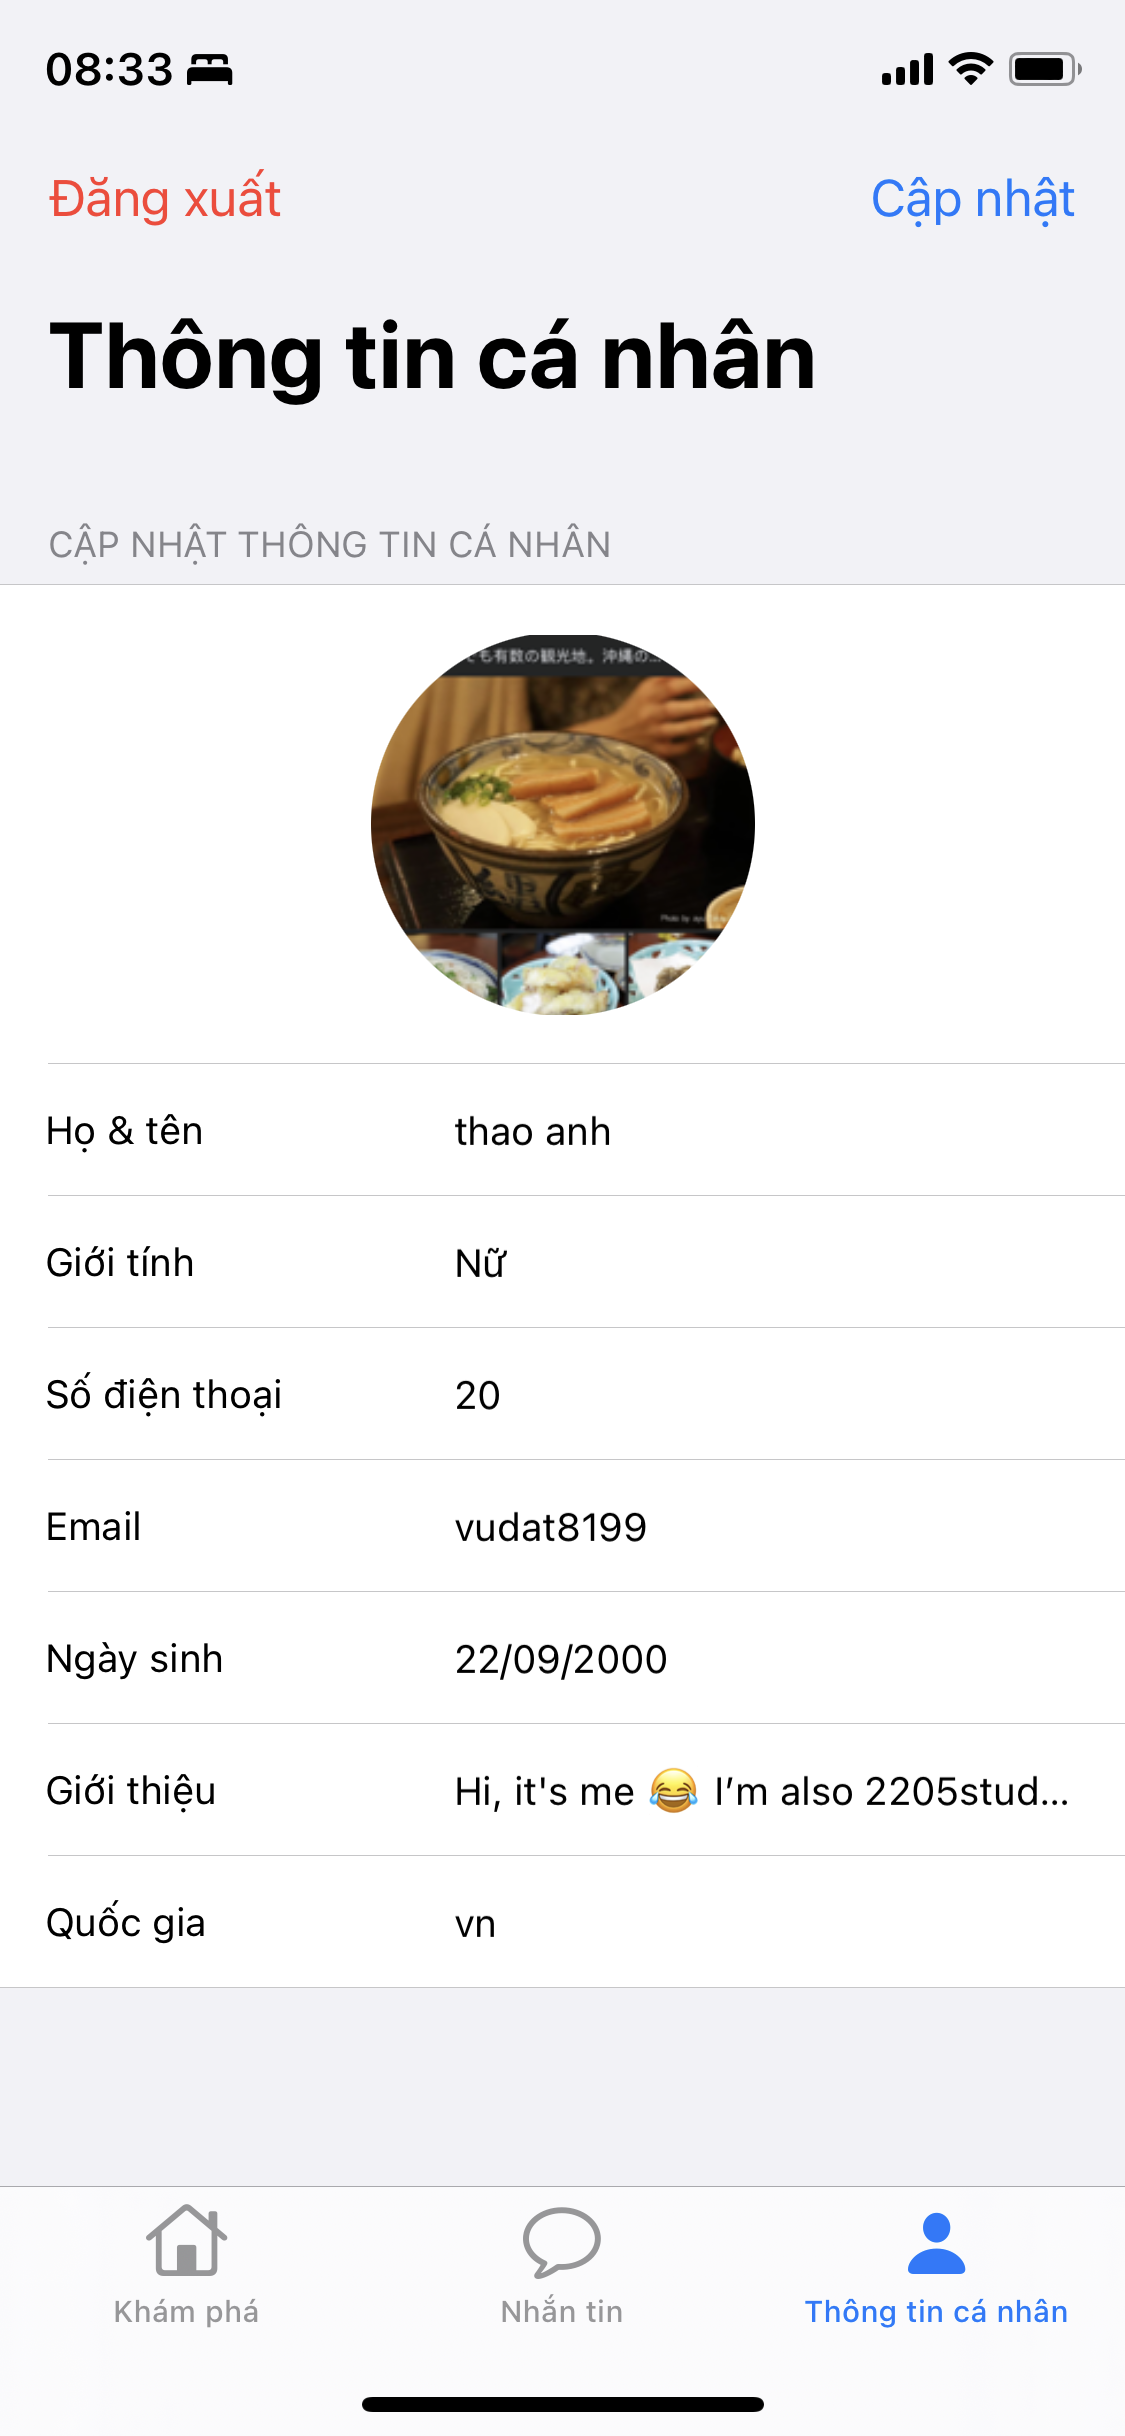
\includegraphics[width=0.95\linewidth]{Hinhve/Application/Private_Profile.png}
\caption{Màn hình xem thông tin bản thân} \label{fig:list_task}
\end{minipage}
\end{figure}

\begin{figure}[H]
\begin{minipage}{0.5\textwidth}
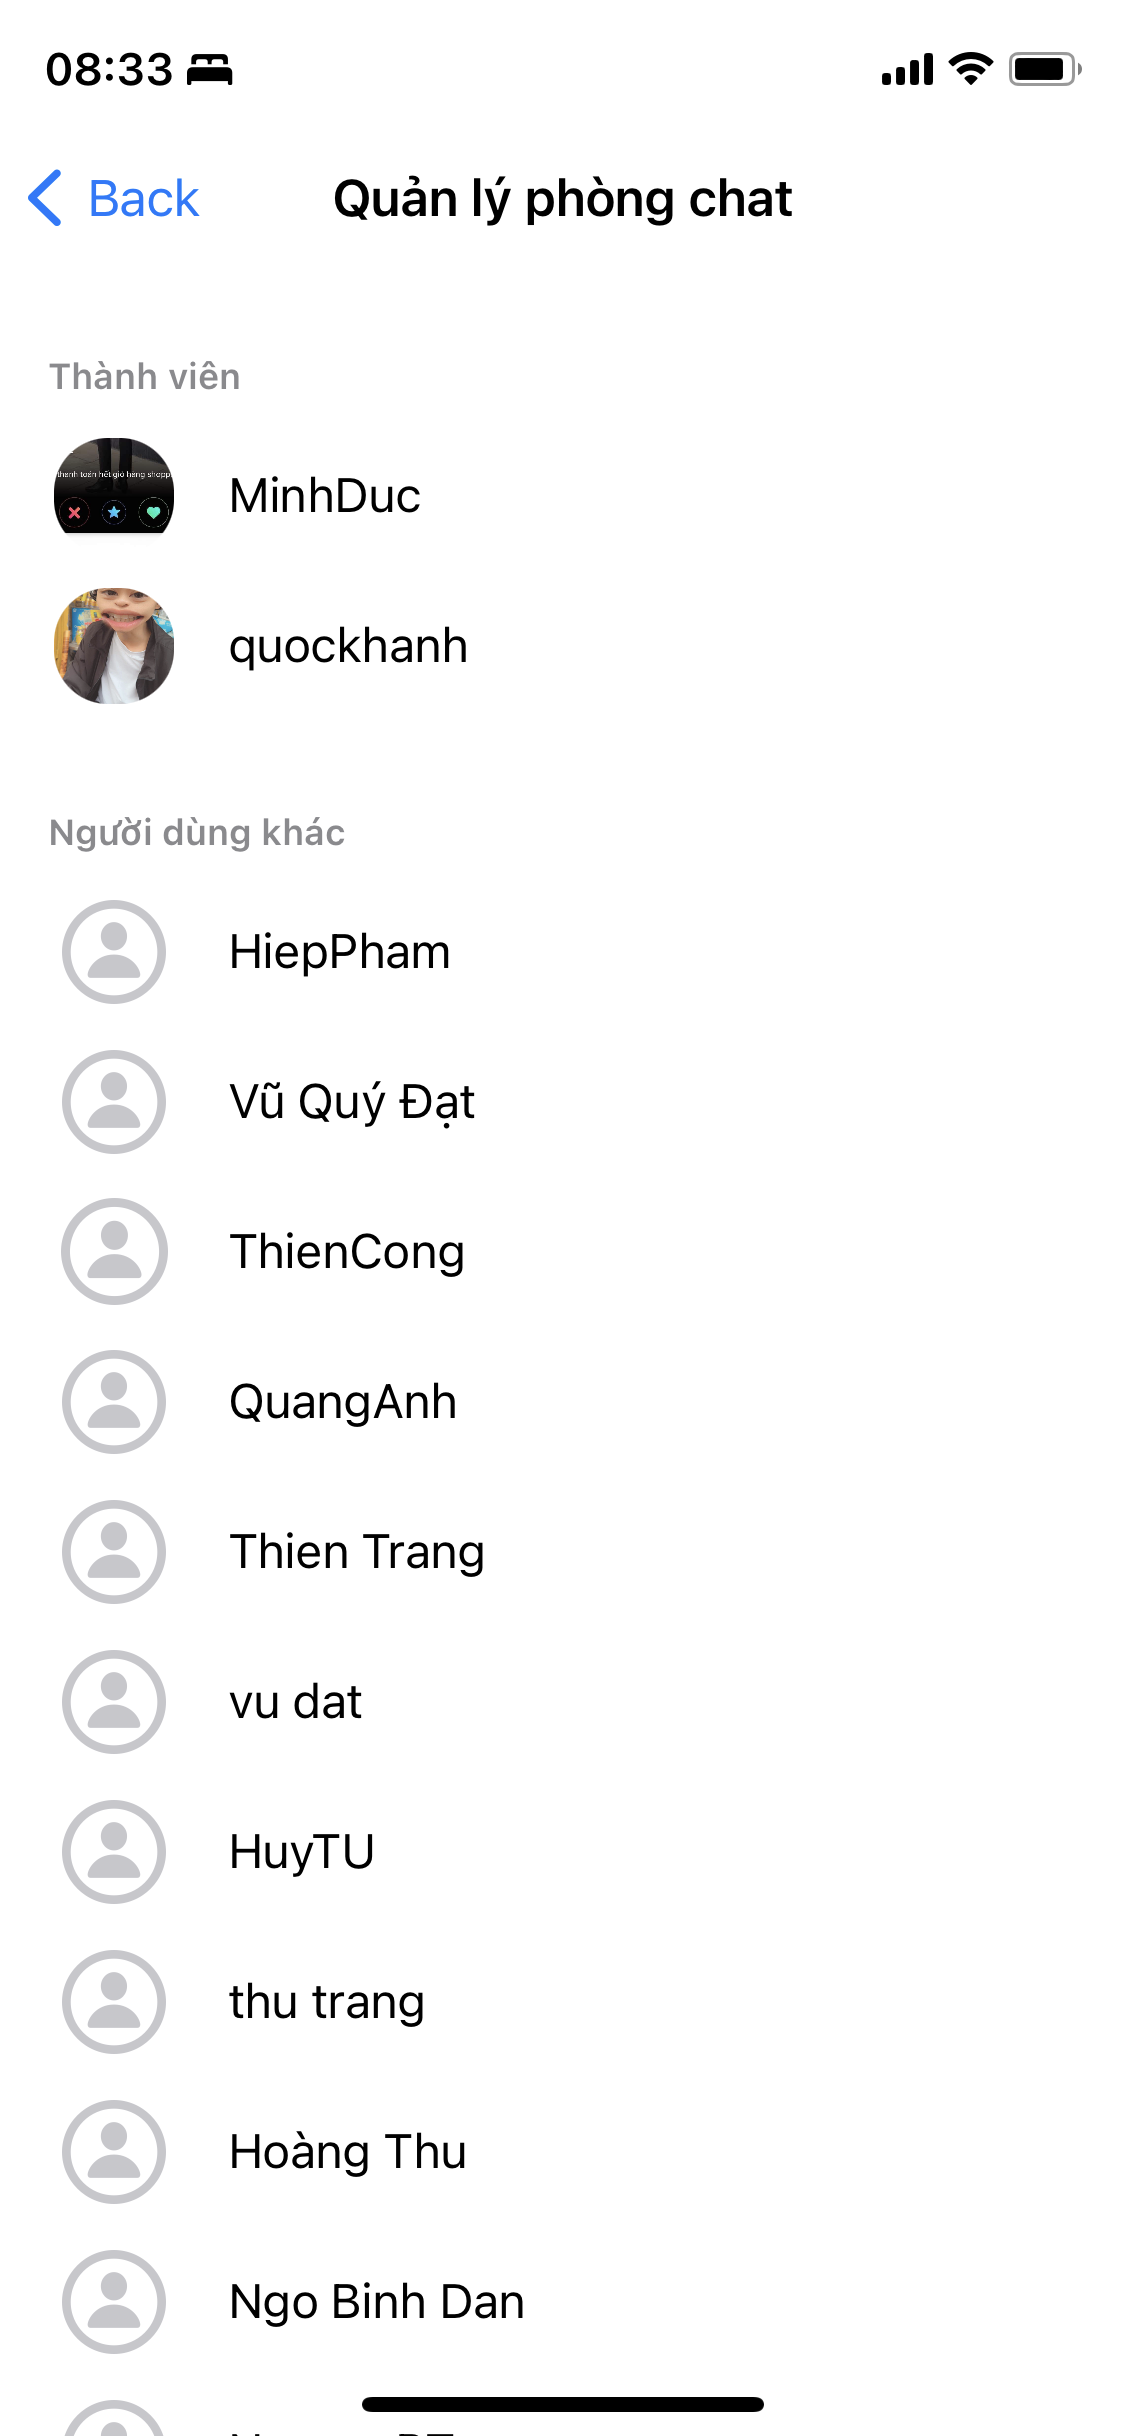
\includegraphics[width=0.95\linewidth]{Hinhve/Application/Managing_Chatbox.png}
\caption{Màn hình quản lý thành viên chat box} \label{fig:screen_login}
\end{minipage}
\hspace{\fill}
\begin{minipage}{0.5\textwidth}
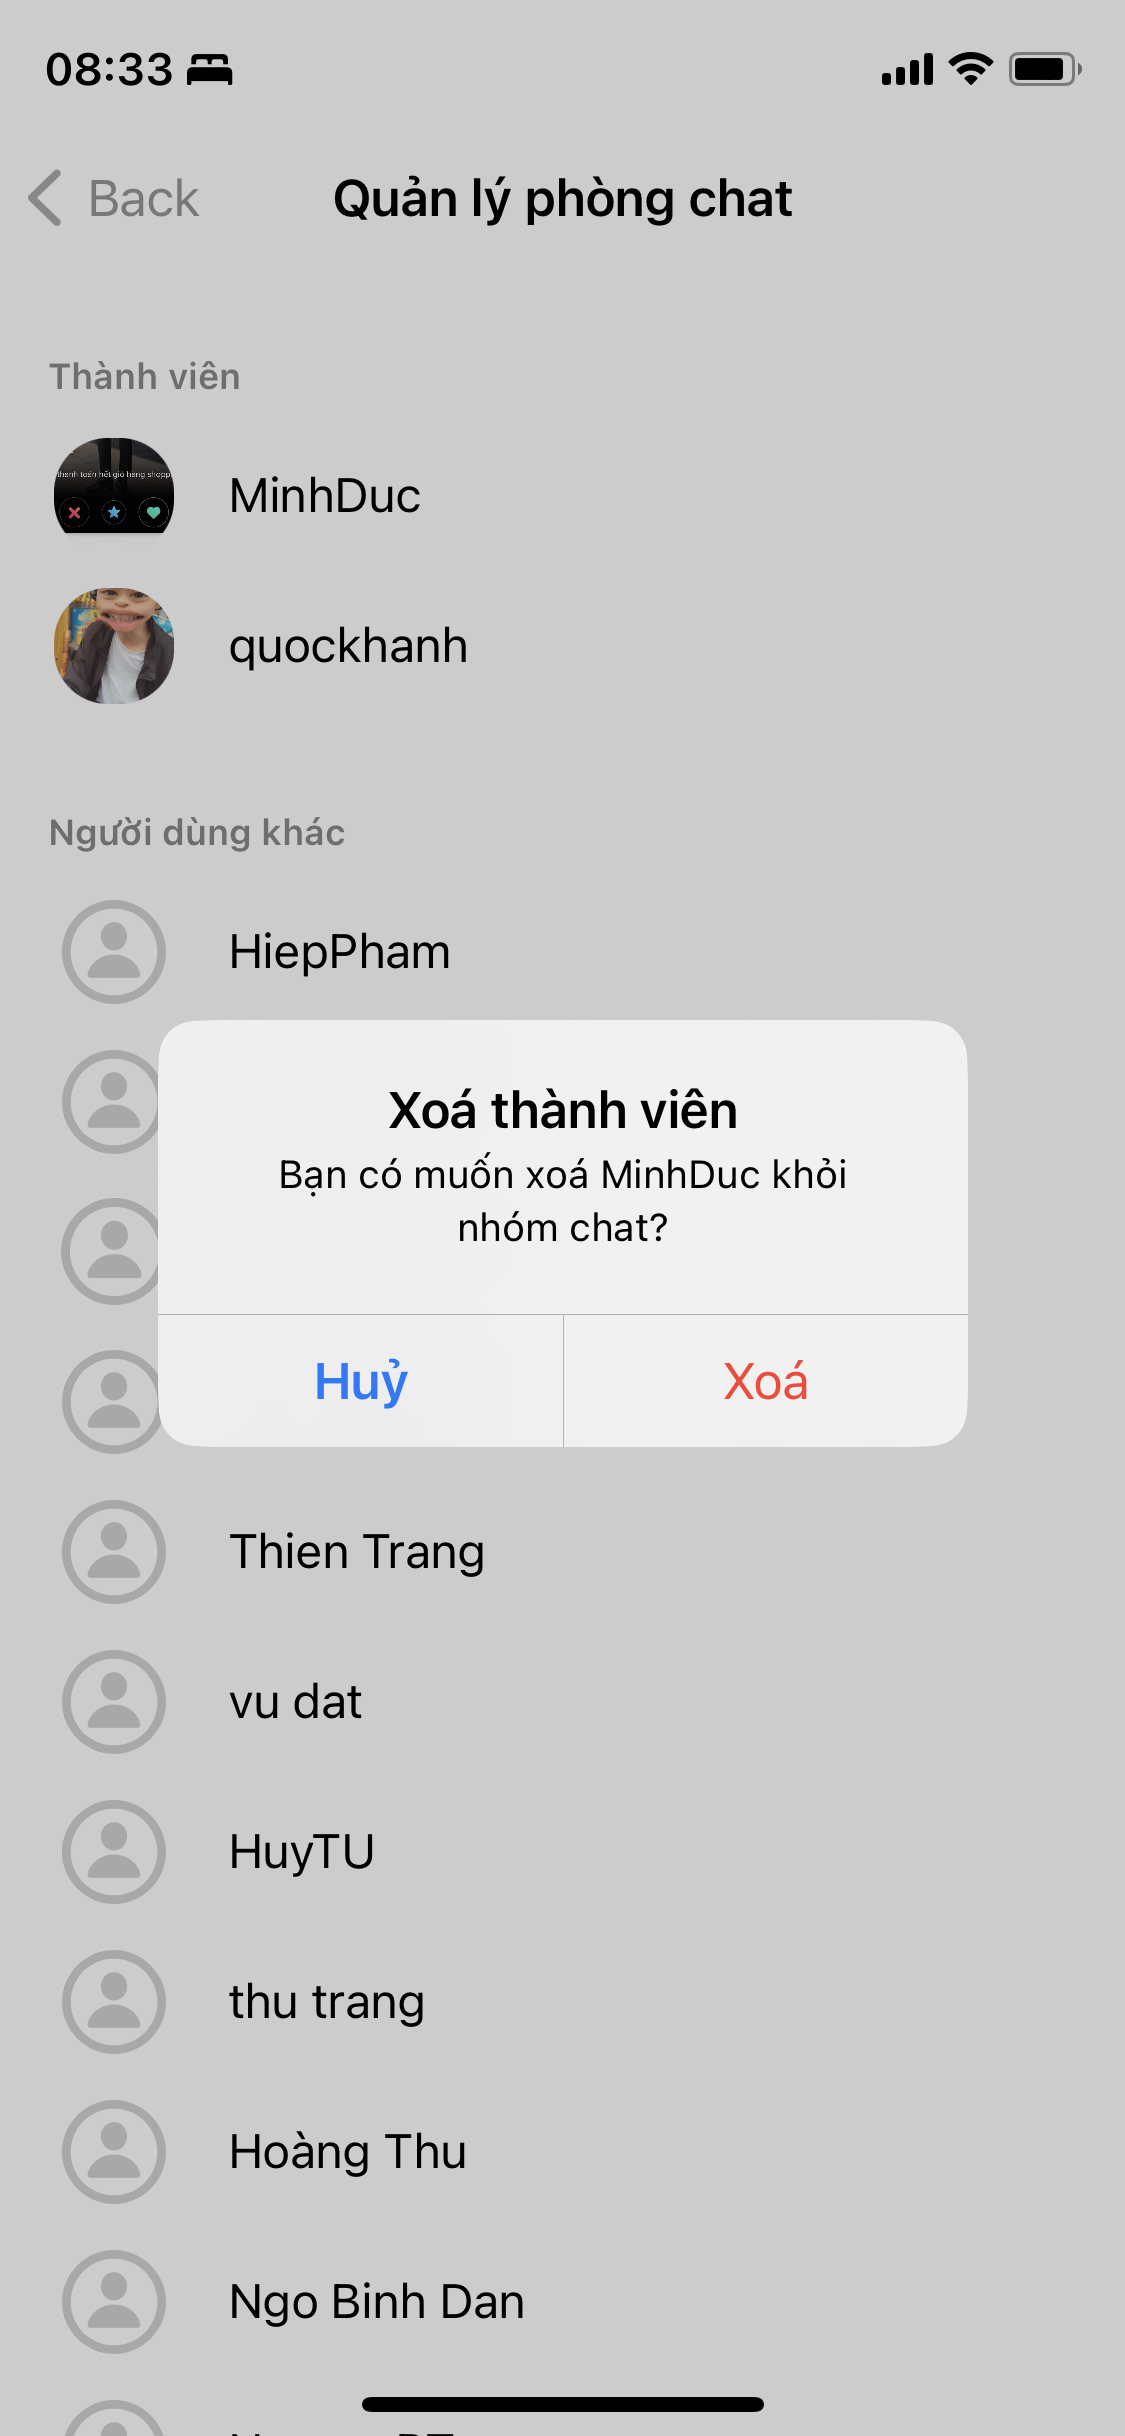
\includegraphics[width=0.95\linewidth]{Hinhve/Application/Managing_Chatbox_Remove_Member.png}
\caption{Màn hình xoá thành viên khỏi chat box} \label{fig:list_task}
\end{minipage}
\end{figure}

\begin{figure}[H]
\begin{minipage}{0.5\textwidth}
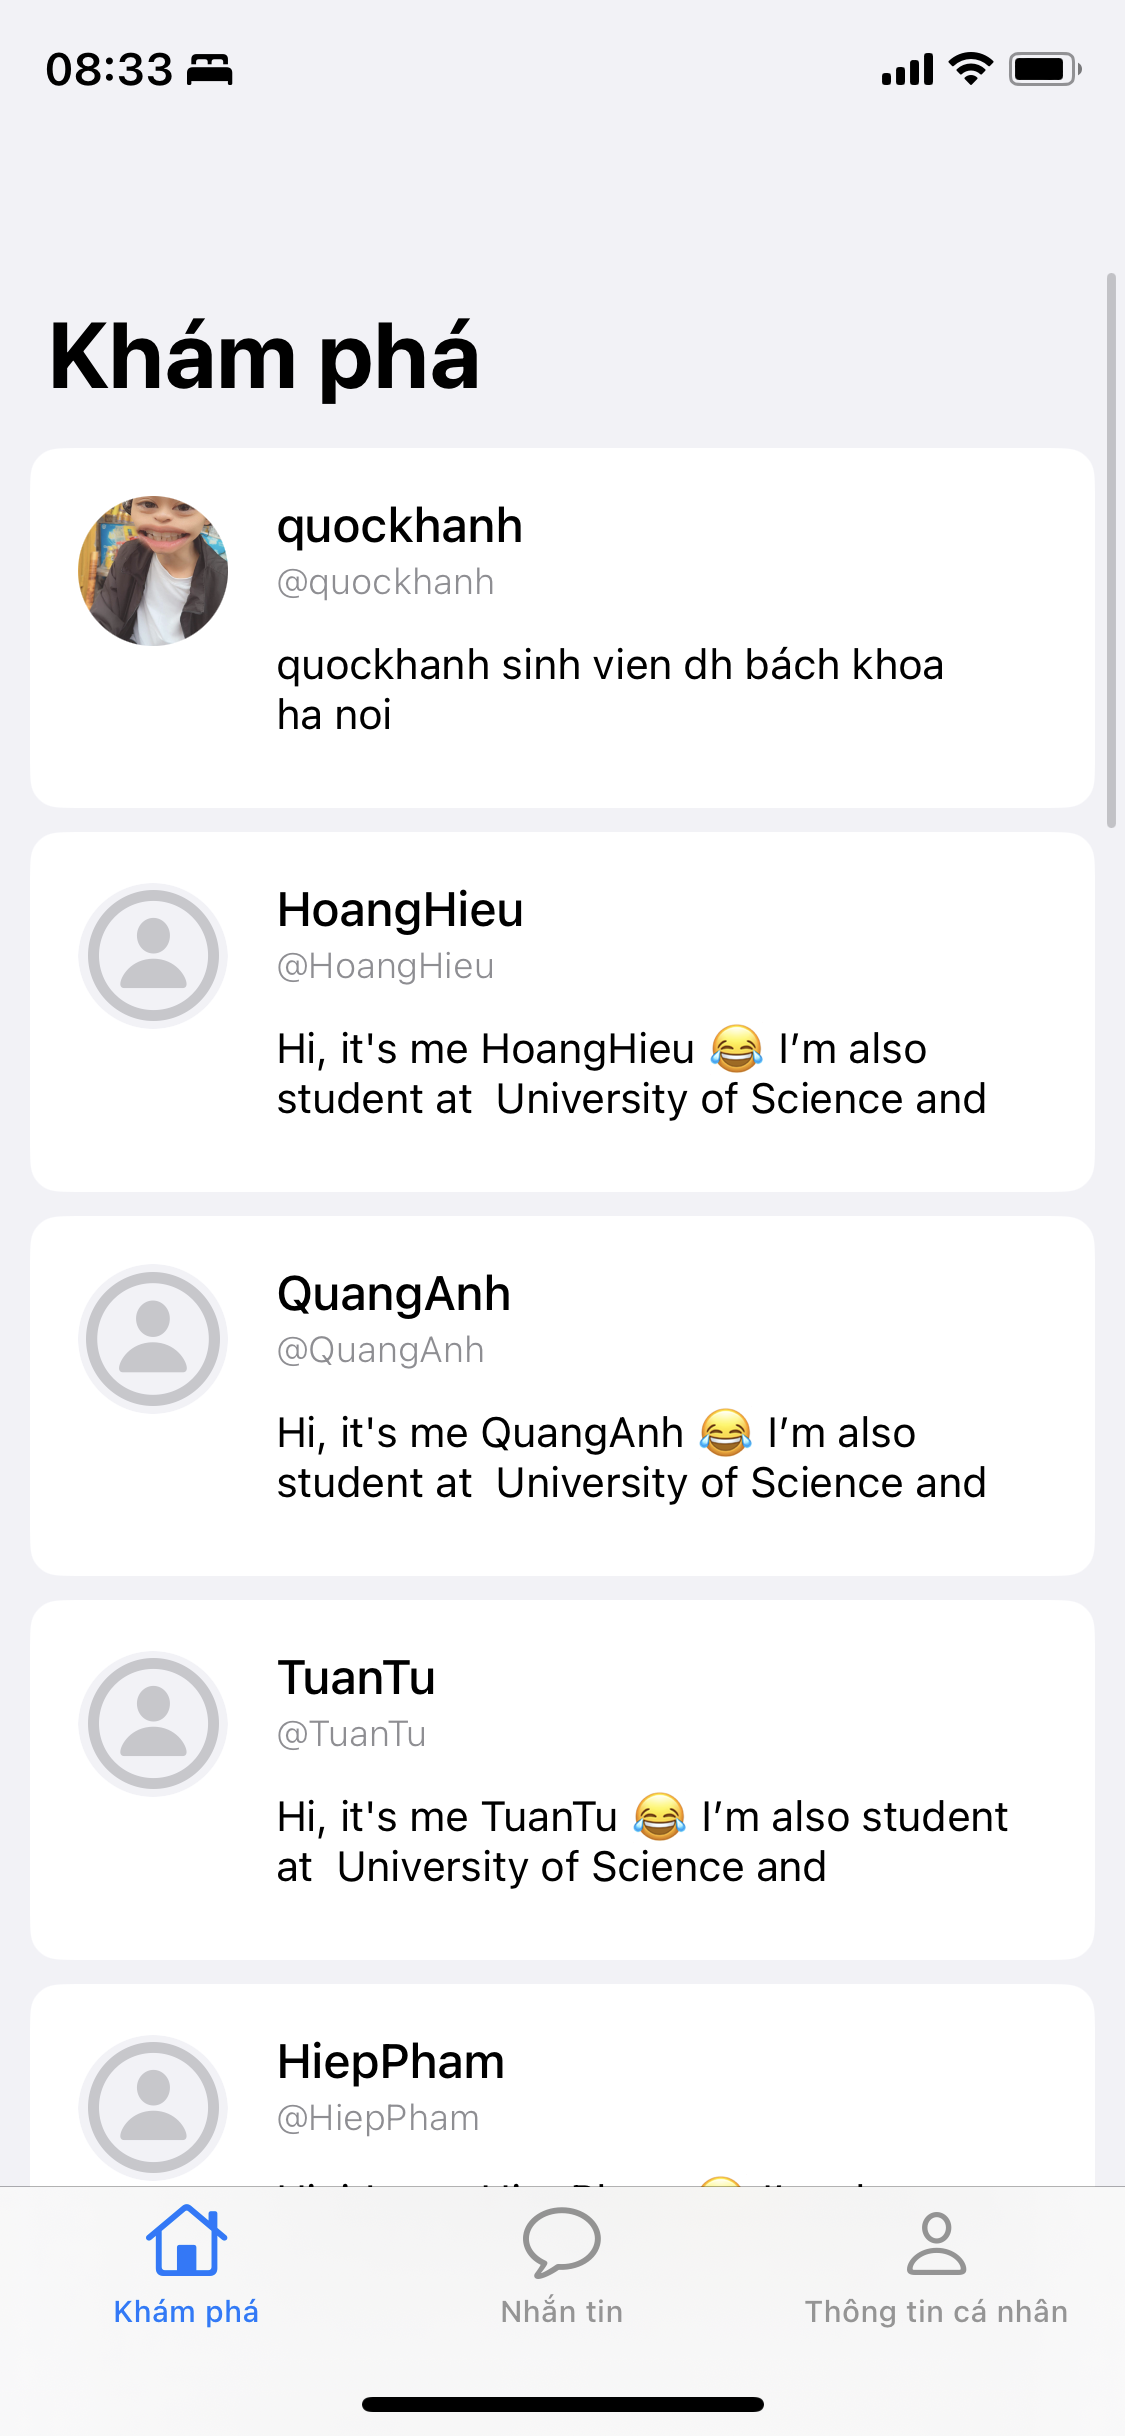
\includegraphics[width=0.95\linewidth]{Hinhve/Application/Explore.png}
\caption{Màn hình danh sách người dùng} \label{fig:screen_login}
\end{minipage}
\hspace{\fill}
\begin{minipage}{0.5\textwidth}
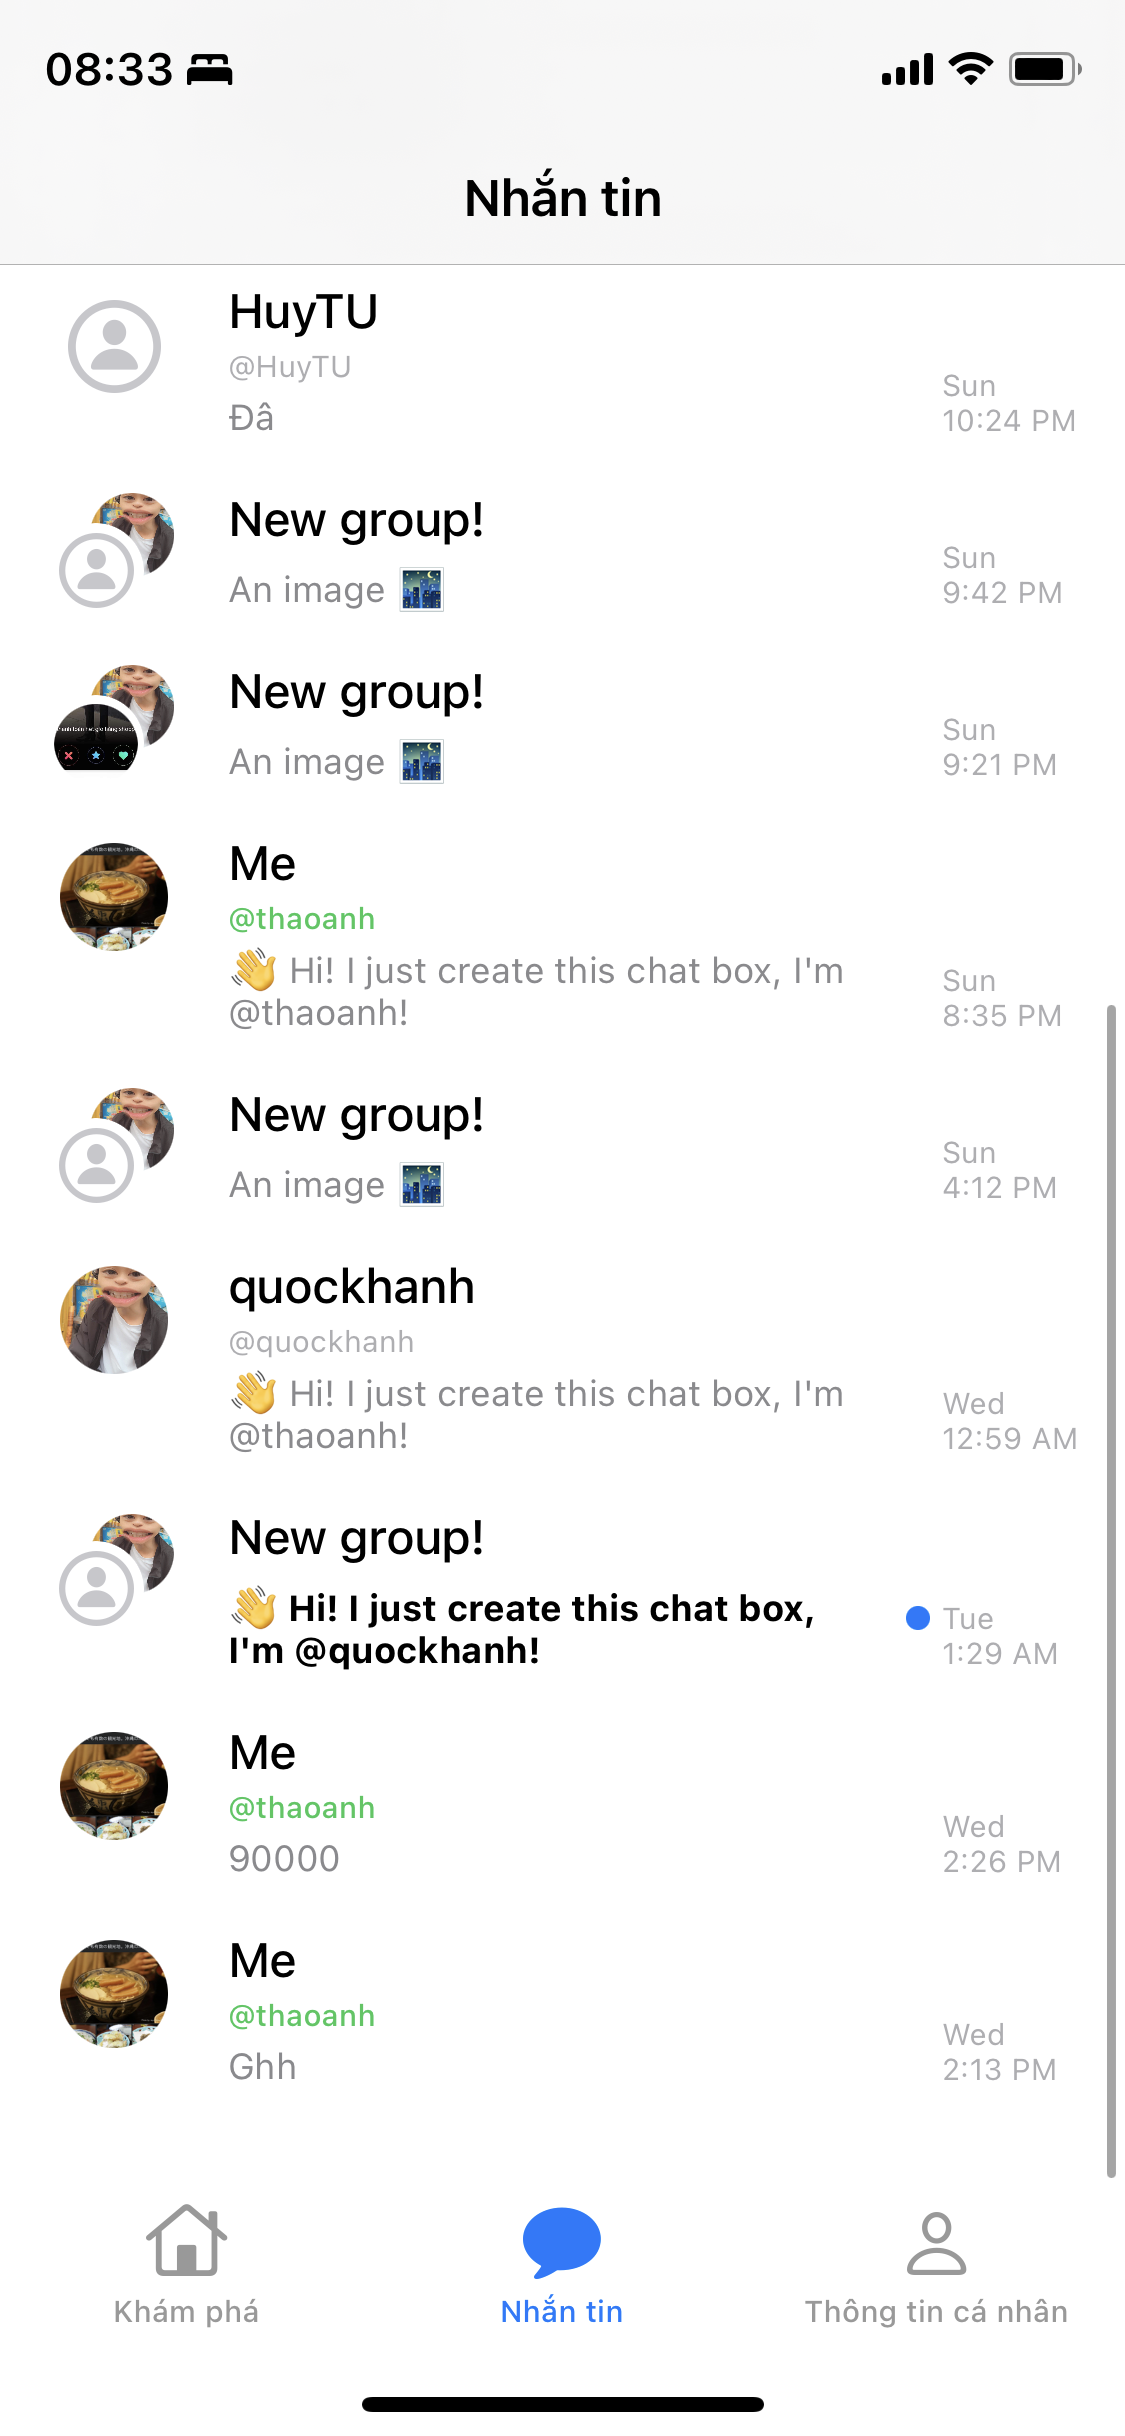
\includegraphics[width=0.95\linewidth]{Hinhve/Application/Chatbox.png}
\caption{Màn hình danh sách chat box} \label{fig:list_task}
\end{minipage}
\end{figure}

\begin{figure}[H]
    \centering
    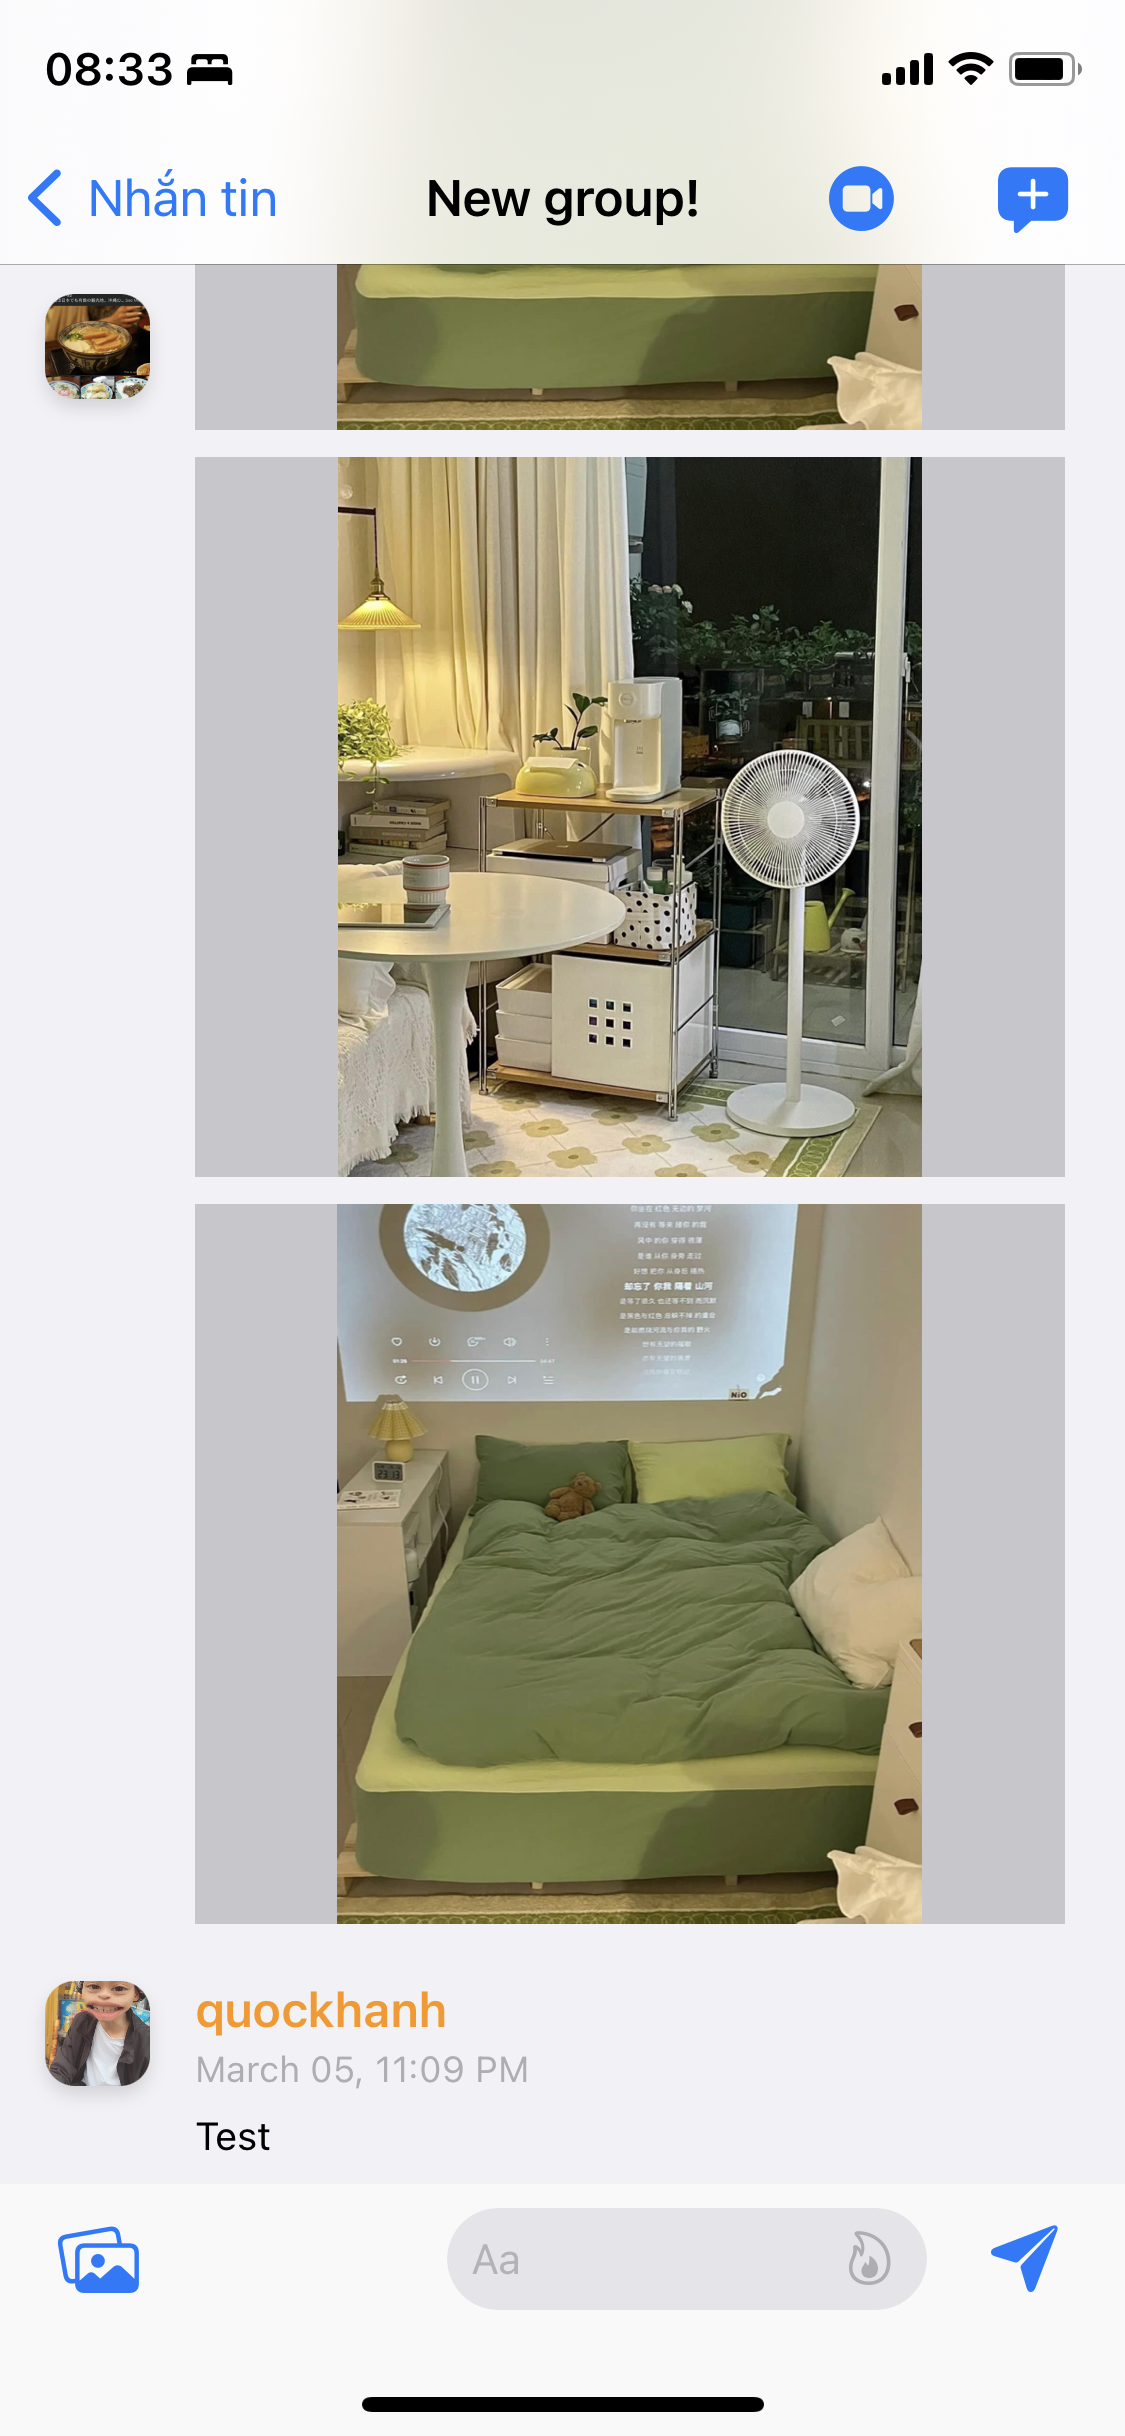
\includegraphics[width=0.5\linewidth]{Hinhve/Application/Messaging.png}
    \caption{Màn hình nhắn tin}
    \label{fig:use_case_tổng_quan}
\end{figure}




\section{Kiểm thử} 
\begin{longtable}[c]{
|>{\raggedright\arraybackslash}m{0.05\linewidth}
|>{\raggedright\arraybackslash}m{0.15\linewidth}
|>{\raggedright\arraybackslash}m{0.3\linewidth}
|>{\raggedright\arraybackslash}m{0.3\linewidth}
|>{\raggedright\arraybackslash}m{0.05\linewidth}|}
\hline
\textbf{STT} & \textbf{Chức năng} & \textbf{Đầu vào} & \textbf{Đầu ra} & \textbf{Kết quả} \hline
\endfirsthead
1 & Đăng ký & Nhập đầy đủ và đúng yêu cầu của các trường bắt buộc & Thông báo đăng ký tài khoàn thành công và hiển thị màn hình đăng nhập & Đạt \\ \hline
2 & Đăng ký & Nhập thiếu các trường bắt buộc & Hiển thị thông báo yêu cầu người dùng kiểm tra lại thông tin tài khoản & Đạt \\ \hline
3 & Đăng nhập & Nhập đúng cả 2 trường với tài khoản và mật khẩu đã tồn tại trong cơ sở dữ liệu & Đăng nhập thành công và hiển thị màn hình chính & Đạt \\ \hline
4 & Đăng nhập & Nhập sai thông tin 1 hoặc cả 2 trường & Hiển thị thông báo yêu cầu người dùng kiểm tra lại tài khoản và mật khẩu & Đạt \\ \hline
5 & Đăng nhập & Nhập thiếu 1 hoặc cả 2 trường & Yêu cầu người dùng kiểm tra lại tài khoản và mật khẩu & Đạt \\ \hline
6 & Đăng xuất & Ấn nút đăng xuất & Xoá dữ liệu người dùng hiện tại và hiển thị màn hình đăng nhập & Đạt \\ \hline
7 & Xem thông tin người dùng & Ấn vào 1 người dùng ở màn hình chính & Hiển thị màn hình thông tin người dùng & Đạt \\ \hline
8 & Tạo phòng chat & Kéo thanh người dùng từ phải sang trái & Phản hồi cho người dùng bằng âm thanh và cập nhật danh sách nhóm chat & Đạt \\ \hline
9 & Gửi tin nhắn văn bản & Nhập tin nhắn văn bản và ấn gửi & Cập nhật tin nhắn mới trên màn hình xem tin nhắn và màn hình danh sách nhóm chat & Đạt \\ \hline
10 & Gửi tin nhắn ảnh & Chọn ảnh muốn gửi và ấn gửi & Cập nhật tin nhắn mới trên màn hình xem tin nhắn và màn hình danh sách nhóm chat & Đạt \\ \hline
11 & Gọi điện video & Ấn vào nút gọi trên màn hình chat & Nhìn thấy video và nghe, nói chuyện được với người đang gọi tới & Đạt \\ \hline
12 & Thêm người dùng vào nhóm chat & Chọn nút thêm trên màn hình chat sau đó chọn người dùng muốn thêm vào nhóm và ấn xác nhận & Cập nhật danh sách người dùng & Đạt \\ \hline
13 & Xoá người dùng khỏi nhóm chat & Chọn nút thêm trên màn hình chat sau đó chọn người dùng muốn xoá khỏi nhóm và ấn xác nhận & Cập nhật danh sách người dùng & Đạt \\ \hline
14 & Rời khỏi nhóm chat & Tại màn hình danh sách nhóm chat, kéo thanh nhóm chat từ phải sang trái và ấn xác nhận & Xoá nhóm chat khỏi danh sách nhóm chat & Đạt \\ \hline
15 & Chỉnh sửa thông tin cá nhân công khai & Chỉnh sửa thông tin bất kỳ sau đó chọn cập nhật trên màn hình thông tin cá nhân & Cập nhật thông tin trên màn hình thông tin cá nhân và phản hổi bằng âm thanh & Đạt \\ \hline
16 & Chỉnh sửa ảnh đại diện & Chọn ảnh bất kỳ sau đó chọn cập nhật trên màn hình thông tin cá nhân & Cập nhật thông tin trên màn hình thông tin cá nhân và phản hổi bằng âm thanh & Đạt \\ \hline
\caption{Kết quả kiểm thử}
\label{tab:use_case_tổng_quan}
\end{longtable}



\section{Triển khai}
Back-end được triển khai trên Docker, phần back-end có thể cài đặt được ở trên nhiều nền tảng, miễn là cài đặt Docker. Dưới đây là các bước cài đặt và triển khai trên MacOS và Ubuntu:

\textbf{Cài đặt:}

Bước 1: Cài đặt Docker.

Cài đặt Docker trên máy chủ ở trang chủ của Docker.

Sau khi cài đặt Docker, mở Docker lên và chạy thử 1 container để kiểm tra bằng cách mở cửa sổ dòng lệnh và chạy:

docker run hello-world

Sau đó chạy:

docker run -it ubuntu bash

Đây là kết quả sau khi chạy:

docker run hello-world

Unable to find image 'hello-world:latest' locally

latest: Pulling from library/hello-world

0e03bdcc26d7: Pull complete

Digest: 

sha256:49a1c8800c94df04e9658809b006fd8a686cab8028d33cfba2cc049724254202

Status: Downloaded newer image for hello-world:latest

docker run -it ubuntu bash

Bước 2: Cấu hình Docker.

Cấu hình PostgreSQL trên Docker:
\begin{itemize}
    \item Tạo file docker-compose.yml tại thư mục Thesis/Back-end.
    \item Thêm đoạn cấu hình sau vào file docker-compose.yml:
        \begin{figure}[H]
            \centering
            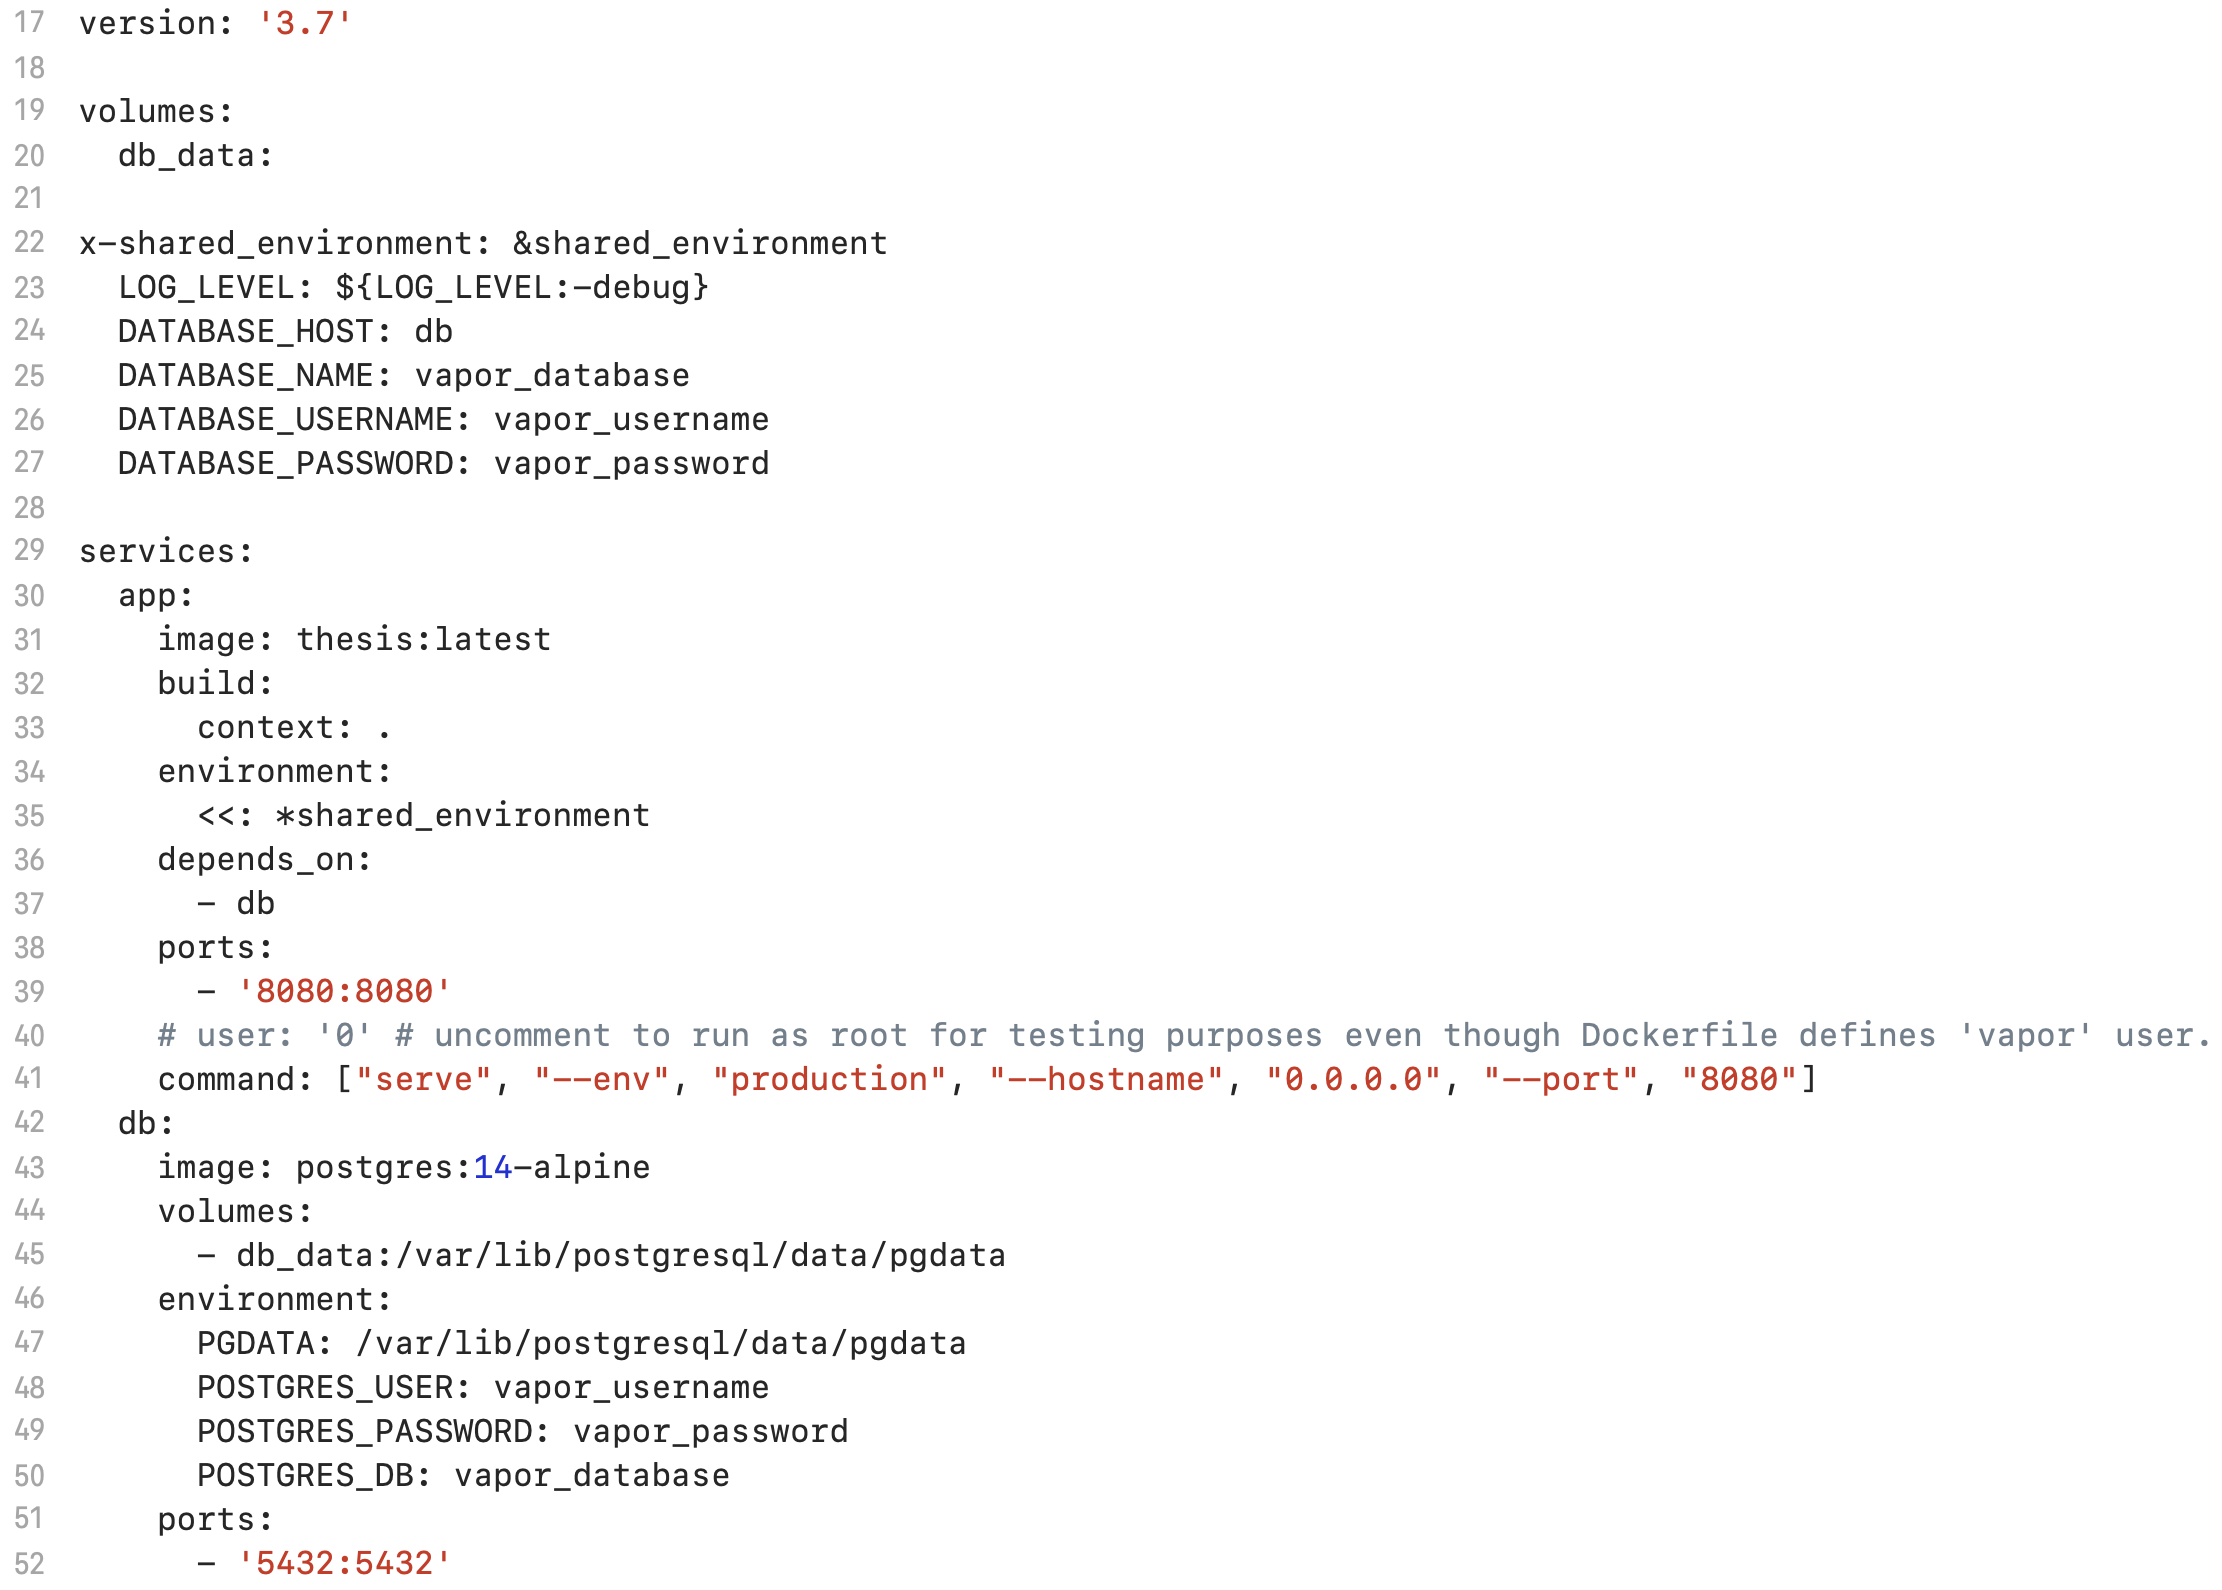
\includegraphics[width=1\linewidth]{Hinhve/Deploy/PostgreSQL.png}
        \end{figure}
    version: '3.7' - là phiên bản của Docker compose

    Phiên bản PostgreSQL sử dụng:
    
    postgres:14-alpine
    
    DATABASE USERNAME: vaporusername - là username của database
    
    POSTGRES PASSWORD: vaporpassword - là mật khẩu của database

    POSTGRES DB: vapordatabase - là tên của database

    Cách cấu hình port forwarding cho PostgreSQL database trên Docker
    
    ports:
    
      - '5432:5432'

    \item Mở cửa sổ dòng lệnh và chạy:
    
    docker-compose up db

    \item Mở Docker References lên và kiểm tra:
        \begin{figure}[H]
            \centering
            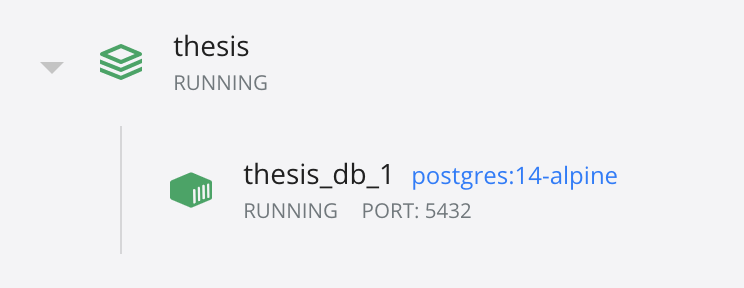
\includegraphics[width=1\linewidth]{Hinhve/Deploy/PostgreSQL_Running_Status.png}  
            \caption{Container thông báo đang chạy PostgreSQL}
            \label{fig:use_case_tổng_quan}
        \end{figure}
    
\end{itemize}

Cấu hình MongoDB trên Docker:
\begin{itemize}
    \item Mở cửa sổ dòng lệnh và chạy:
    
    docker run --name mongodb -d -p 27017:27017 mongo
    
    \item Mở Docker References lên và kiểm tra:
        \begin{figure}[H]
            \centering
            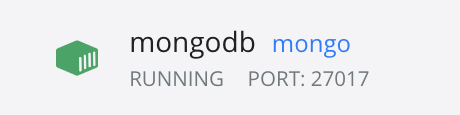
\includegraphics[width=1\linewidth]{Hinhve/Deploy/MongoDB_Running_Status.png}  
            \caption{Container thông báo đang chạy MongoDB}
            \label{fig:use_case_tổng_quan}
        \end{figure}
        
\end{itemize}

Bước 3: Cấu hình HTTP server.

Từ thư mục mã nguồn của đồ án, vào đường dẫn Thesis/Back-end, Tại đây thư mục Signaling là phần service cho tính năng gọi video trực tuyến, các thư mục còn lại dùng để triển khai http server và websocket.

Triển khai http server trên MacOS: 

\begin{itemize}
    \item Từ thư mục Back-end, mở mã nguồn trên XCode IDE bằng cách mở file Package.swift.
    \item Cấu hình http server trong file configure.swift:

    Cấu hình ip

    let host = "192.168.1.24"

    Cấu hình port

    app.http.server.configuration.port = 8080

    Cấu hình dung lượng lớn nhất của http body
    
    app.routes.defaultMaxBodySize = "20mb"

    Cấu hình tên database

    databaseName = "vapordatabase"

    Cấu hình port database

    databasePort = 5432

    Cấu hình hostname database

    hostname: Environment.get("DATABASEHOST") ?? "localhost"

    Cấu hình username database
    
    username: Environment.get("DATABASEUSERNAME") ?? "vaporusername"


    Cấu hình password database
    
    password: Environment.get("DATABASEPASSWORD") ?? "vaporpassword"

    Cấu hình MongoDB

    try app.databases.use(.mongo(connectionString: "mongodb://localhost:27017/mongo"), as: .mongo)

    try app.initializeMongoDB(connectionString: "mongodb://localhost:27017/mongo")

    \item Bắt đầu chạy phần mềm trên Xcode bằng tổ hợp phím command + R
\end{itemize}


Triển khai http server trên Ubuntu:

Cấu hình server trên Ubunto giống với hướng dẫn trên MacOS.

Chạy phần mềm trên Ubuntu:

\begin{itemize}
    \item Mở cửa sổ dòng lệnh và bắt đầu cài đặt Swift bằng lệnh sau:
    sudo apt install clang libpython2.7 libpython2.7-dev
    
    wget https://swift.org/builds/swift-5.3-release/ubuntu2004/swift-5.3-RELEASE/swift-5.3-RELEASE-ubuntu20.04.tar.gz
    
    tar xzf swift-5.3-RELEASE-ubuntu20.04.tar.gz
    
    sudo mv swift-5.3-RELEASE-ubuntu20.04 /usr/share/swift

    % Nhớ thêm dấu $ trước PATH: echo "export PATH=/usr/share/swift/usr/bin:$PATH" >> ~/.zshrc
    echo "export PATH=/usr/share/swift/usr/bin:PATH" >> ~/.zshrc 
    
    source ~/.zshrc

    \item Sau khi đã cài đặt xong Swift, chay lệnh sau để bắt đầu biên dịch mã nguồn:
    
    swift build

    \item Sau khi biên dịch thành công, chạy lệnh sau để chạy phần mềm với ip và port được chỉ định:

    swift run Run --hostname 192.168.1.24 --port 8080

\end{itemize}

Bước 4: Chạy signaling server phục vụ cho tính năng gọi điện video trực tuyến.
\begin{itemize}
    \item Từ thư mục Back-end, trỏ vào thư mục signaling từ cửa sổ dòng lệnh, chạy lệnh:
    
    swiftc main.swift WebSocketServer.swift WebSocketClient.swift -o server
    
    ./server

    \item server sẽ bắt đầu chạy.
\end{itemize}

Bước 5: Cài đặt ứng dụng trên iOS.
\begin{itemize}
    \item Từ thư mục mã nguồn của đồ án Thesis, mở thư mục ChatApp sau đó mở file ChatApp.xcodeproj.
    
    \item Sửa mục nhà phát triển thành nhóm phát triển đính kém với tài khoản Apple iCloud.

    \item Chạy phần mềm bằng tổ hợp phím command + R.
\end{itemize}



% \begin{longtable}[c]{
% |>{\raggedright\arraybackslash}m{0.25\linewidth}
% |>{\raggedright\arraybackslash}m{0.15\linewidth}
% |>{\raggedright\arraybackslash}m{0.20\linewidth}
% |>{\raggedright\arraybackslash}m{0.20\linewidth}|}

% \hline
% \centering \textbf{Chức năng} & \centering \textbf{Shopee} & \centering \textbf{daohaisan.vn} \hline
% \endfirsthead

% Hệ thống nâng cấp tài khoản cá nhân thành tài khoản cộng tác viên mua hàng giá rẻ. & Chưa có & Chưa có  \\ \hline
% Hệ thống bình luận, đánh giá sản phẩm & Chưa tối ưu, nhiều bình luận rác, khiến điểm đánh giá chưa được chính xác & Đã tối ưu  \\ \hline
% Gợi ý sản phẩm theo thói quen người dùng & Có & Chưa có  \\ \hline
% Hệ thống giỏ hàng được đồng bộ theo tài khoản & Chưa giải quyết vấn đề lưu trữ khi chưa đăng nhập & Có  \\ \hline
% Hệ thống thanh toán online & Có & Có \\ \hline

% \caption{So sánh chức năng giữa các hệ thống website bán hàng trên thị trường}
% \label{tab:use_case_tổng_quan}

% \end{longtable}





% \section{Thiết kế kiến trúc}
% \subsection{Lựa chọn kiến trúc phần mềm}
% Mục này có độ dài từ một đến ba trang. Sinh viên cần lựa chọn kiến trúc phần mềm cho ứng dụng của mình như: kiến trúc ba lớp MVC, MVP, SOA, Microservice, v.v. rồi giải thích sơ bộ về kiến trúc đó (không giải thích chi tiết/dài dòng).
% Sử dụng kiến trúc phần mềm đã chọn ở trên, sinh viên mô tả kiến trúc cụ thể cho ứng dụng của mình. Gợi ý: sinh viên áp dụng lý thuyết chung vào hệ thống/sản phẩm của mình như thế nào, có thay đổi, bổ sung hoặc cải tiến gì không. Ví dụ, thành phần M trong kiến trúc lý thuyết MVC sẽ là những thành phần cụ thể nào (ví dụ: là interface I + class C1 + class C2, v.v.) trong kiến trúc phần mềm của sinh viên.

% \subsection{Thiết kế tổng quan}
% Sinh viên vẽ biểu đồ gói UML (UML package diagram), nêu rõ sự phụ thuộc giữa các gói (package). SV cần vẽ các gói sao cho chúng được phân theo các tầng rõ ràng, không được sắp đặt package lộn xộn trong hình vẽ. Sinh viên chú ý các quy tắc thiết kế (Các gói không phụ thuộc lẫn nhau, gói tầng dưới không phụ thuộc gói tầng trên, không phụ thuộc bỏ qua tầng, v.v.) và cần giải thích sơ lược về mục đích/nhiệm vụ của từng package. SV tham khảo ví dụ minh họa trong Hình \ref{fig:Fig1}
% \begin{figure}[H]
%     \centering
%     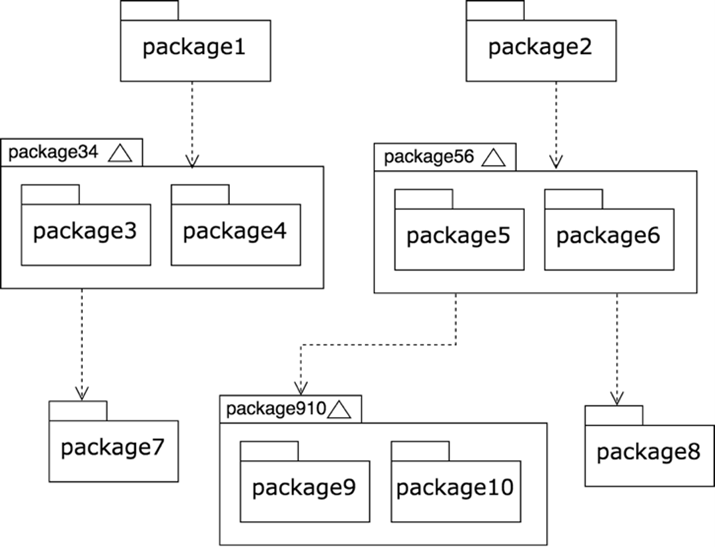
\includegraphics{Hinhve/Picture1.png}
%     \caption{Ví dụ biểu đồ phụ thuộc gói}
%     \label{fig:Fig1}
% \end{figure}
% \subsection{Thiết kế chi tiết gói}
% Sinh viên thiết kế và lần lượt vẽ biểu đồ thiết kế cho từng package, hoặc một nhóm các package liên quan để giải quyết một vấn đề gì đó. Khi vẽ thiết kế gói, sinh viên chỉ cần đưa tên lớp, không cần chỉ ra các thành viên phương thức và thuộc tính. SV tham khảo ví dụ minh họa trong Hình \ref{fig:Fig2}.

% Sinh viên cần vẽ rõ ràng quan hệ giữa các lớp trong biểu đồ. Các quan hệ bao gồm: phụ thuộc (dependency), kết hợp (association), kết tập (aggregation), hợp thành (composition), kế thừa (inheritance), và thực thi (implementation). Các quan hệ này đều đã được minh họa trong \ref{fig:Fig2}.

% Sau khi vẽ hình minh họa, sinh viên cần giải thích ngắn gọn về thiết kế của mình. 

% \begin{figure}[H]
%     \centering
%     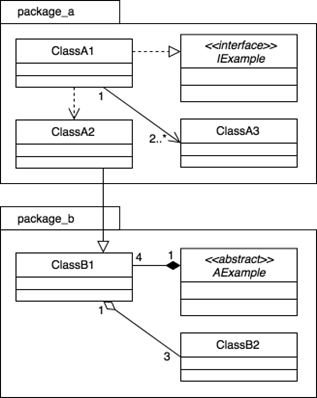
\includegraphics{Hinhve/Picture2.png}
%     \caption{Ví dụ thiết kế gói}
%     \label{fig:Fig2}
% \end{figure}

% \section{Thiết kế chi tiết}
% \subsection{Thiết kế giao diện}
% Phần này có độ dài từ hai đến ba trang. Sinh viên đặc tả thông tin về màn hình mà ứng dụng của mình hướng tới, bao gồm độ phân giải màn hình, kích thước màn hình, số lượng màu sắc hỗ trợ, v.v. Tiếp đến, sinh viên đưa ra các thống nhất/chuẩn hóa của mình khi thiết kế giao diện như thiết kế nút, điều khiển, vị trí hiển thị thông điệp phản hồi, phối màu, v.v. Sau cùng sinh viên đưa ra một số hình ảnh minh họa thiết kế giao diện cho các chức năng quan trọng nhất. Lưu ý, sinh viên không nhầm lẫn giao diện thiết kế với giao diện của sản phẩm sau cùng.
% \subsection{Thiết kế lớp}
% Phần này có độ dài từ ba đến bốn trang. Sinh viên trình bày thiết kế chi tiết các thuộc tính và phương thức cho một số lớp chủ đạo/quan trọng nhất của ứng dụng (từ 2-4 lớp). Thiết kế chi tiết cho các lớp khác, nếu muốn trình bày, sinh viên đưa vào phần phụ lục.

% Để minh họa thiết kế lớp, sinh viên thiết kế luồng truyền thông điệp giữa các đối tượng tham gia cho 2 đến 3 use case quan trọng nào đó bằng biểu đồ trình tự (hoặc biểu đồ giao tiếp).
% \subsection{Thiết kế cơ sở dữ liệu}
% Phần này có độ dài từ hai đến bốn trang. Sinh viên thiết kế, vẽ và giải thích biểu đồ thực thể liên kết (E-R diagram). Từ đó, sinh viên thiết kế cơ sở dữ liệu tùy theo hệ quản trị cơ sở dữ liệu mà mình sử dụng (SQL, NoSQL, Firebase, v.v.)

% \section{Xây dựng ứng dụng}
% \subsection{Thư viện và công cụ sử dụng}
% Sinh viên liệt kê các công cụ, ngôn ngữ lập trình, API, thư viện, IDE, công cụ kiểm thử, v.v. mà mình sử dụng để phát triển ứng dụng. Mỗi công cụ phải được chỉ rõ phiên bản sử dụng. SV nên kẻ bảng mô tả tương tự như Bảng \ref{table:my_label}. Nếu có nhiều nội dung trình bày, sinh viên cần xoay ngang bảng.

% \begin{table}[H]
% \centering{}
%     \begin{tabular}{lll}
%         \hline
%         \textbf{Mục đích} & \textbf{Công cụ}       & \textbf{Địa chỉ URL}    \\ \hline
%         IDE lập trình     & Eclipse Oxygen a64 bit & http://www.eclipse.org/ \\ \hline
%         v.v.              & v.v.                   & v.v.                    \\ \hline
%         \end{tabular}
%     \caption{Danh sách thư viện và công cụ sử dụng}
%     \label{fig:my_label}
% \end{table}

% \subsection{Kết quả đạt được}
% Sinh viên trước tiên mô tả kết quả đạt được của mình là gì, ví dụ như các sản phẩm được đóng gói là gì, bao gồm những thành phần nào, ý nghĩa, vai trò?

% Sinh viên cần thống kê các thông tin về ứng dụng của mình như: số dòng code, số lớp, số gói, dung lượng toàn bộ mã nguồn, dung lượng của từng sản phẩm đóng gói, v.v. Tương tự như phần liệt kê về công cụ sử dụng, sinh viên cũng nên dùng bảng để mô tả phần thông tin thống kê này.

% \subsection{Minh họa các chức năng chính}
% Sinh viên lựa chọn và đưa ra màn hình cho các chức năng chính, quan trọng, và thú vị nhất. Mỗi giao diện cần phải có lời giải thích ngắn gọn. Khi giải thích, sinh viên có thể kết hợp với các chú thích ở trong hình ảnh giao diện.

% \section{Kiểm thử}
% Phần này có độ dài từ hai đến ba trang. Sinh viên thiết kế các trường hợp kiểm thử cho hai đến ba chức năng quan trọng nhất. Sinh viên cần chỉ rõ các kỹ thuật kiểm thử đã sử dụng. Chi tiết các trường hợp kiểm thử khác, nếu muốn trình bày, sinh viên đưa vào phần phụ lục.
% Sinh viên sau cùng tổng kết về số lượng các trường hợp kiểm thử và kết quả kiểm thử. Sinh viên cần phân tích lý do nếu kết quả kiểm thử không đạt.
% \section{Triển khai}
% Sinh viên trình bày mô hình và/hoặc cách thức triển khai thử nghiệm/thực tế. Ứng dụng của sinh viên được triển khai trên server/thiết bị gì, cấu hình như thế nào. Kết quả triển khai thử nghiệm nếu có (số lượng người dùng, số lượng truy cập, thời gian phản hồi, phản hồi người dùng, khả năng chịu tải, các thống kê, v.v.)

\end{document}
